\documentclass{book}
\usepackage[a4paper,top=2.5cm,bottom=2.5cm,left=2.5cm,right=2.5cm]{geometry}
\usepackage{makeidx}
\usepackage{natbib}
\usepackage{graphicx}
\usepackage{multicol}
\usepackage{float}
\usepackage{listings}
\usepackage{color}
\usepackage{ifthen}
\usepackage[table]{xcolor}
\usepackage{textcomp}
\usepackage{alltt}
\usepackage{ifpdf}
\ifpdf
\usepackage[pdftex,
            pagebackref=true,
            colorlinks=true,
            linkcolor=blue,
            unicode
           ]{hyperref}
\else
\usepackage[ps2pdf,
            pagebackref=true,
            colorlinks=true,
            linkcolor=blue,
            unicode
           ]{hyperref}
\usepackage{pspicture}
\fi
\usepackage[utf8]{inputenc}
\usepackage{mathptmx}
\usepackage[scaled=.90]{helvet}
\usepackage{courier}
\usepackage{sectsty}
\usepackage{amssymb}
\usepackage[titles]{tocloft}
\usepackage{doxygen}
\lstset{language=C++,inputencoding=utf8,basicstyle=\footnotesize,breaklines=true,breakatwhitespace=true,tabsize=4,numbers=left }
\makeindex
\setcounter{tocdepth}{3}
\renewcommand{\footrulewidth}{0.4pt}
\renewcommand{\familydefault}{\sfdefault}
\hfuzz=15pt
\setlength{\emergencystretch}{15pt}
\hbadness=750
\tolerance=750
\begin{document}
\hypersetup{pageanchor=false,citecolor=blue}
\begin{titlepage}
\vspace*{7cm}
\begin{center}
{\Large Record\-Studio }\\
\vspace*{1cm}
{\large Generated by Doxygen 1.8.3.1}\\
\vspace*{0.5cm}
{\small Sat Aug 31 2013 09:56:10}\\
\end{center}
\end{titlepage}
\clearemptydoublepage
\pagenumbering{roman}
\tableofcontents
\clearemptydoublepage
\pagenumbering{arabic}
\hypersetup{pageanchor=true,citecolor=blue}
\chapter{Hierarchical Index}
\section{Class Hierarchy}
This inheritance list is sorted roughly, but not completely, alphabetically\-:\begin{DoxyCompactList}
\item \contentsline{section}{B\-A\-S\-S\-\_\-3\-D\-V\-E\-C\-T\-O\-R}{\pageref{struct_b_a_s_s__3_d_v_e_c_t_o_r}}{}
\item \contentsline{section}{B\-A\-S\-S\-\_\-\-C\-H\-A\-N\-N\-E\-L\-I\-N\-F\-O}{\pageref{struct_b_a_s_s___c_h_a_n_n_e_l_i_n_f_o}}{}
\item \contentsline{section}{B\-A\-S\-S\-\_\-\-D\-E\-V\-I\-C\-E\-I\-N\-F\-O}{\pageref{struct_b_a_s_s___d_e_v_i_c_e_i_n_f_o}}{}
\item \contentsline{section}{B\-A\-S\-S\-\_\-\-D\-X8\-\_\-\-C\-H\-O\-R\-U\-S}{\pageref{struct_b_a_s_s___d_x8___c_h_o_r_u_s}}{}
\item \contentsline{section}{B\-A\-S\-S\-\_\-\-D\-X8\-\_\-\-C\-O\-M\-P\-R\-E\-S\-S\-O\-R}{\pageref{struct_b_a_s_s___d_x8___c_o_m_p_r_e_s_s_o_r}}{}
\item \contentsline{section}{B\-A\-S\-S\-\_\-\-D\-X8\-\_\-\-D\-I\-S\-T\-O\-R\-T\-I\-O\-N}{\pageref{struct_b_a_s_s___d_x8___d_i_s_t_o_r_t_i_o_n}}{}
\item \contentsline{section}{B\-A\-S\-S\-\_\-\-D\-X8\-\_\-\-E\-C\-H\-O}{\pageref{struct_b_a_s_s___d_x8___e_c_h_o}}{}
\item \contentsline{section}{B\-A\-S\-S\-\_\-\-D\-X8\-\_\-\-F\-L\-A\-N\-G\-E\-R}{\pageref{struct_b_a_s_s___d_x8___f_l_a_n_g_e_r}}{}
\item \contentsline{section}{B\-A\-S\-S\-\_\-\-D\-X8\-\_\-\-G\-A\-R\-G\-L\-E}{\pageref{struct_b_a_s_s___d_x8___g_a_r_g_l_e}}{}
\item \contentsline{section}{B\-A\-S\-S\-\_\-\-D\-X8\-\_\-\-I3\-D\-L2\-R\-E\-V\-E\-R\-B}{\pageref{struct_b_a_s_s___d_x8___i3_d_l2_r_e_v_e_r_b}}{}
\item \contentsline{section}{B\-A\-S\-S\-\_\-\-D\-X8\-\_\-\-P\-A\-R\-A\-M\-E\-Q}{\pageref{struct_b_a_s_s___d_x8___p_a_r_a_m_e_q}}{}
\item \contentsline{section}{B\-A\-S\-S\-\_\-\-D\-X8\-\_\-\-R\-E\-V\-E\-R\-B}{\pageref{struct_b_a_s_s___d_x8___r_e_v_e_r_b}}{}
\item \contentsline{section}{B\-A\-S\-S\-\_\-\-F\-I\-L\-E\-P\-R\-O\-C\-S}{\pageref{struct_b_a_s_s___f_i_l_e_p_r_o_c_s}}{}
\item \contentsline{section}{B\-A\-S\-S\-\_\-\-I\-N\-F\-O}{\pageref{struct_b_a_s_s___i_n_f_o}}{}
\item \contentsline{section}{B\-A\-S\-S\-\_\-\-M\-I\-X\-E\-R\-\_\-\-N\-O\-D\-E}{\pageref{struct_b_a_s_s___m_i_x_e_r___n_o_d_e}}{}
\item \contentsline{section}{B\-A\-S\-S\-\_\-\-P\-L\-U\-G\-I\-N\-F\-O\-R\-M}{\pageref{struct_b_a_s_s___p_l_u_g_i_n_f_o_r_m}}{}
\item \contentsline{section}{B\-A\-S\-S\-\_\-\-P\-L\-U\-G\-I\-N\-I\-N\-F\-O}{\pageref{struct_b_a_s_s___p_l_u_g_i_n_i_n_f_o}}{}
\item \contentsline{section}{B\-A\-S\-S\-\_\-\-R\-E\-C\-O\-R\-D\-I\-N\-F\-O}{\pageref{struct_b_a_s_s___r_e_c_o_r_d_i_n_f_o}}{}
\item \contentsline{section}{B\-A\-S\-S\-\_\-\-S\-A\-M\-P\-L\-E}{\pageref{struct_b_a_s_s___s_a_m_p_l_e}}{}
\item \contentsline{section}{M\-S\-Master\-Splitter}{\pageref{class_m_s_master_splitter}}{}
\item Q\-Exception\begin{DoxyCompactList}
\item \contentsline{section}{D\-A\-W\-Inputs\-:\-:D\-A\-W\-Error}{\pageref{class_d_a_w_inputs_1_1_d_a_w_error}}{}
\item \contentsline{section}{M\-S\-Master\-Error}{\pageref{class_m_s_master_error}}{}
\end{DoxyCompactList}
\item Q\-Object\begin{DoxyCompactList}
\item \contentsline{section}{D\-A\-W\-Inputs\-:\-:Input\-Base}{\pageref{class_d_a_w_inputs_1_1_input_base}}{}
\begin{DoxyCompactList}
\item \contentsline{section}{D\-A\-W\-Inputs\-:\-:File\-Input}{\pageref{class_d_a_w_inputs_1_1_file_input}}{}
\end{DoxyCompactList}
\end{DoxyCompactList}
\item \contentsline{section}{T\-A\-G\-\_\-\-A\-P\-E\-\_\-\-B\-I\-N\-A\-R\-Y}{\pageref{struct_t_a_g___a_p_e___b_i_n_a_r_y}}{}
\item \contentsline{section}{T\-A\-G\-\_\-\-B\-E\-X\-T}{\pageref{struct_t_a_g___b_e_x_t}}{}
\item \contentsline{section}{T\-A\-G\-\_\-\-C\-A\-\_\-\-C\-O\-D\-E\-C}{\pageref{struct_t_a_g___c_a___c_o_d_e_c}}{}
\item \contentsline{section}{T\-A\-G\-\_\-\-C\-A\-R\-T}{\pageref{struct_t_a_g___c_a_r_t}}{}
\item \contentsline{section}{T\-A\-G\-\_\-\-C\-A\-R\-T\-\_\-\-T\-I\-M\-E\-R}{\pageref{struct_t_a_g___c_a_r_t___t_i_m_e_r}}{}
\item \contentsline{section}{T\-A\-G\-\_\-\-I\-D3}{\pageref{struct_t_a_g___i_d3}}{}
\item \contentsline{section}{t\-W\-A\-V\-E\-F\-O\-R\-M\-A\-T\-E\-X}{\pageref{structt_w_a_v_e_f_o_r_m_a_t_e_x}}{}
\end{DoxyCompactList}

\chapter{Class Index}
\section{Class List}
Here are the classes, structs, unions and interfaces with brief descriptions\-:\begin{DoxyCompactList}
\item\contentsline{section}{\hyperlink{struct_b_a_s_s__3_d_v_e_c_t_o_r}{B\-A\-S\-S\-\_\-3\-D\-V\-E\-C\-T\-O\-R} }{\pageref{struct_b_a_s_s__3_d_v_e_c_t_o_r}}{}
\item\contentsline{section}{\hyperlink{struct_b_a_s_s___c_h_a_n_n_e_l_i_n_f_o}{B\-A\-S\-S\-\_\-\-C\-H\-A\-N\-N\-E\-L\-I\-N\-F\-O} }{\pageref{struct_b_a_s_s___c_h_a_n_n_e_l_i_n_f_o}}{}
\item\contentsline{section}{\hyperlink{struct_b_a_s_s___d_e_v_i_c_e_i_n_f_o}{B\-A\-S\-S\-\_\-\-D\-E\-V\-I\-C\-E\-I\-N\-F\-O} }{\pageref{struct_b_a_s_s___d_e_v_i_c_e_i_n_f_o}}{}
\item\contentsline{section}{\hyperlink{struct_b_a_s_s___d_x8___c_h_o_r_u_s}{B\-A\-S\-S\-\_\-\-D\-X8\-\_\-\-C\-H\-O\-R\-U\-S} }{\pageref{struct_b_a_s_s___d_x8___c_h_o_r_u_s}}{}
\item\contentsline{section}{\hyperlink{struct_b_a_s_s___d_x8___c_o_m_p_r_e_s_s_o_r}{B\-A\-S\-S\-\_\-\-D\-X8\-\_\-\-C\-O\-M\-P\-R\-E\-S\-S\-O\-R} }{\pageref{struct_b_a_s_s___d_x8___c_o_m_p_r_e_s_s_o_r}}{}
\item\contentsline{section}{\hyperlink{struct_b_a_s_s___d_x8___d_i_s_t_o_r_t_i_o_n}{B\-A\-S\-S\-\_\-\-D\-X8\-\_\-\-D\-I\-S\-T\-O\-R\-T\-I\-O\-N} }{\pageref{struct_b_a_s_s___d_x8___d_i_s_t_o_r_t_i_o_n}}{}
\item\contentsline{section}{\hyperlink{struct_b_a_s_s___d_x8___e_c_h_o}{B\-A\-S\-S\-\_\-\-D\-X8\-\_\-\-E\-C\-H\-O} }{\pageref{struct_b_a_s_s___d_x8___e_c_h_o}}{}
\item\contentsline{section}{\hyperlink{struct_b_a_s_s___d_x8___f_l_a_n_g_e_r}{B\-A\-S\-S\-\_\-\-D\-X8\-\_\-\-F\-L\-A\-N\-G\-E\-R} }{\pageref{struct_b_a_s_s___d_x8___f_l_a_n_g_e_r}}{}
\item\contentsline{section}{\hyperlink{struct_b_a_s_s___d_x8___g_a_r_g_l_e}{B\-A\-S\-S\-\_\-\-D\-X8\-\_\-\-G\-A\-R\-G\-L\-E} }{\pageref{struct_b_a_s_s___d_x8___g_a_r_g_l_e}}{}
\item\contentsline{section}{\hyperlink{struct_b_a_s_s___d_x8___i3_d_l2_r_e_v_e_r_b}{B\-A\-S\-S\-\_\-\-D\-X8\-\_\-\-I3\-D\-L2\-R\-E\-V\-E\-R\-B} }{\pageref{struct_b_a_s_s___d_x8___i3_d_l2_r_e_v_e_r_b}}{}
\item\contentsline{section}{\hyperlink{struct_b_a_s_s___d_x8___p_a_r_a_m_e_q}{B\-A\-S\-S\-\_\-\-D\-X8\-\_\-\-P\-A\-R\-A\-M\-E\-Q} }{\pageref{struct_b_a_s_s___d_x8___p_a_r_a_m_e_q}}{}
\item\contentsline{section}{\hyperlink{struct_b_a_s_s___d_x8___r_e_v_e_r_b}{B\-A\-S\-S\-\_\-\-D\-X8\-\_\-\-R\-E\-V\-E\-R\-B} }{\pageref{struct_b_a_s_s___d_x8___r_e_v_e_r_b}}{}
\item\contentsline{section}{\hyperlink{struct_b_a_s_s___f_i_l_e_p_r_o_c_s}{B\-A\-S\-S\-\_\-\-F\-I\-L\-E\-P\-R\-O\-C\-S} }{\pageref{struct_b_a_s_s___f_i_l_e_p_r_o_c_s}}{}
\item\contentsline{section}{\hyperlink{struct_b_a_s_s___i_n_f_o}{B\-A\-S\-S\-\_\-\-I\-N\-F\-O} }{\pageref{struct_b_a_s_s___i_n_f_o}}{}
\item\contentsline{section}{\hyperlink{struct_b_a_s_s___m_i_x_e_r___n_o_d_e}{B\-A\-S\-S\-\_\-\-M\-I\-X\-E\-R\-\_\-\-N\-O\-D\-E} }{\pageref{struct_b_a_s_s___m_i_x_e_r___n_o_d_e}}{}
\item\contentsline{section}{\hyperlink{struct_b_a_s_s___p_l_u_g_i_n_f_o_r_m}{B\-A\-S\-S\-\_\-\-P\-L\-U\-G\-I\-N\-F\-O\-R\-M} }{\pageref{struct_b_a_s_s___p_l_u_g_i_n_f_o_r_m}}{}
\item\contentsline{section}{\hyperlink{struct_b_a_s_s___p_l_u_g_i_n_i_n_f_o}{B\-A\-S\-S\-\_\-\-P\-L\-U\-G\-I\-N\-I\-N\-F\-O} }{\pageref{struct_b_a_s_s___p_l_u_g_i_n_i_n_f_o}}{}
\item\contentsline{section}{\hyperlink{struct_b_a_s_s___r_e_c_o_r_d_i_n_f_o}{B\-A\-S\-S\-\_\-\-R\-E\-C\-O\-R\-D\-I\-N\-F\-O} }{\pageref{struct_b_a_s_s___r_e_c_o_r_d_i_n_f_o}}{}
\item\contentsline{section}{\hyperlink{struct_b_a_s_s___s_a_m_p_l_e}{B\-A\-S\-S\-\_\-\-S\-A\-M\-P\-L\-E} }{\pageref{struct_b_a_s_s___s_a_m_p_l_e}}{}
\item\contentsline{section}{\hyperlink{class_d_a_w_inputs_1_1_d_a_w_error}{D\-A\-W\-Inputs\-::\-D\-A\-W\-Error} \\*The \hyperlink{class_d_a_w_inputs_1_1_d_a_w_error}{D\-A\-W\-Error} class }{\pageref{class_d_a_w_inputs_1_1_d_a_w_error}}{}
\item\contentsline{section}{\hyperlink{class_d_a_w_inputs_1_1_file_input}{D\-A\-W\-Inputs\-::\-File\-Input} \\*The \hyperlink{class_d_a_w_inputs_1_1_file_input}{File\-Input} class }{\pageref{class_d_a_w_inputs_1_1_file_input}}{}
\item\contentsline{section}{\hyperlink{class_d_a_w_inputs_1_1_input_base}{D\-A\-W\-Inputs\-::\-Input\-Base} }{\pageref{class_d_a_w_inputs_1_1_input_base}}{}
\item\contentsline{section}{\hyperlink{class_m_s_master_error}{M\-S\-Master\-Error} \\*Thrown by the M\-S\-Master\-Components. Contains Information about the errors occured in those components }{\pageref{class_m_s_master_error}}{}
\item\contentsline{section}{\hyperlink{class_m_s_master_splitter}{M\-S\-Master\-Splitter} \\*Uses a mixer to create a stereo stream that at the left channel mixes the sideband and at the right the midband(the mono signal). The resulting stream is send to a splitterstream that creates two outputstreams(0=S, 1=M) }{\pageref{class_m_s_master_splitter}}{}
\item\contentsline{section}{\hyperlink{struct_t_a_g___a_p_e___b_i_n_a_r_y}{T\-A\-G\-\_\-\-A\-P\-E\-\_\-\-B\-I\-N\-A\-R\-Y} }{\pageref{struct_t_a_g___a_p_e___b_i_n_a_r_y}}{}
\item\contentsline{section}{\hyperlink{struct_t_a_g___b_e_x_t}{T\-A\-G\-\_\-\-B\-E\-X\-T} }{\pageref{struct_t_a_g___b_e_x_t}}{}
\item\contentsline{section}{\hyperlink{struct_t_a_g___c_a___c_o_d_e_c}{T\-A\-G\-\_\-\-C\-A\-\_\-\-C\-O\-D\-E\-C} }{\pageref{struct_t_a_g___c_a___c_o_d_e_c}}{}
\item\contentsline{section}{\hyperlink{struct_t_a_g___c_a_r_t}{T\-A\-G\-\_\-\-C\-A\-R\-T} }{\pageref{struct_t_a_g___c_a_r_t}}{}
\item\contentsline{section}{\hyperlink{struct_t_a_g___c_a_r_t___t_i_m_e_r}{T\-A\-G\-\_\-\-C\-A\-R\-T\-\_\-\-T\-I\-M\-E\-R} }{\pageref{struct_t_a_g___c_a_r_t___t_i_m_e_r}}{}
\item\contentsline{section}{\hyperlink{struct_t_a_g___i_d3}{T\-A\-G\-\_\-\-I\-D3} }{\pageref{struct_t_a_g___i_d3}}{}
\item\contentsline{section}{\hyperlink{structt_w_a_v_e_f_o_r_m_a_t_e_x}{t\-W\-A\-V\-E\-F\-O\-R\-M\-A\-T\-E\-X} }{\pageref{structt_w_a_v_e_f_o_r_m_a_t_e_x}}{}
\end{DoxyCompactList}

\chapter{Class Documentation}
\hypertarget{struct_b_a_s_s__3_d_v_e_c_t_o_r}{\section{B\-A\-S\-S\-\_\-3\-D\-V\-E\-C\-T\-O\-R Struct Reference}
\label{struct_b_a_s_s__3_d_v_e_c_t_o_r}\index{B\-A\-S\-S\-\_\-3\-D\-V\-E\-C\-T\-O\-R@{B\-A\-S\-S\-\_\-3\-D\-V\-E\-C\-T\-O\-R}}
}


Collaboration diagram for B\-A\-S\-S\-\_\-3\-D\-V\-E\-C\-T\-O\-R\-:\nopagebreak
\begin{figure}[H]
\begin{center}
\leavevmode
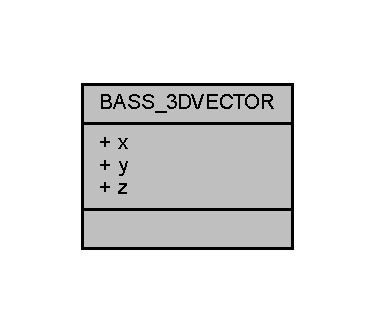
\includegraphics[width=180pt]{struct_b_a_s_s__3_d_v_e_c_t_o_r__coll__graph}
\end{center}
\end{figure}
\subsection*{Public Attributes}
\begin{DoxyCompactItemize}
\item 
\hypertarget{struct_b_a_s_s__3_d_v_e_c_t_o_r_af3d4cc65c06996e789da1c5c295039b1_af3d4cc65c06996e789da1c5c295039b1}{float {\bfseries x}}\label{struct_b_a_s_s__3_d_v_e_c_t_o_r_af3d4cc65c06996e789da1c5c295039b1_af3d4cc65c06996e789da1c5c295039b1}

\item 
\hypertarget{struct_b_a_s_s__3_d_v_e_c_t_o_r_a4284c81914926f579e3e1dde7ad06926_a4284c81914926f579e3e1dde7ad06926}{float {\bfseries y}}\label{struct_b_a_s_s__3_d_v_e_c_t_o_r_a4284c81914926f579e3e1dde7ad06926_a4284c81914926f579e3e1dde7ad06926}

\item 
\hypertarget{struct_b_a_s_s__3_d_v_e_c_t_o_r_a183f698058d7394590cba43e0735a110_a183f698058d7394590cba43e0735a110}{float {\bfseries z}}\label{struct_b_a_s_s__3_d_v_e_c_t_o_r_a183f698058d7394590cba43e0735a110_a183f698058d7394590cba43e0735a110}

\end{DoxyCompactItemize}


\subsection{Detailed Description}


Definition at line 366 of file bass.\-h.



The documentation for this struct was generated from the following files\-:\begin{DoxyCompactItemize}
\item 
D\-A\-W\-Components/bass.\-h\item 
M\-S\-Master\-Cmp/bass.\-h\end{DoxyCompactItemize}

\hypertarget{struct_b_a_s_s___c_h_a_n_n_e_l_i_n_f_o}{\section{B\-A\-S\-S\-\_\-\-C\-H\-A\-N\-N\-E\-L\-I\-N\-F\-O Struct Reference}
\label{struct_b_a_s_s___c_h_a_n_n_e_l_i_n_f_o}\index{B\-A\-S\-S\-\_\-\-C\-H\-A\-N\-N\-E\-L\-I\-N\-F\-O@{B\-A\-S\-S\-\_\-\-C\-H\-A\-N\-N\-E\-L\-I\-N\-F\-O}}
}


Collaboration diagram for B\-A\-S\-S\-\_\-\-C\-H\-A\-N\-N\-E\-L\-I\-N\-F\-O\-:\nopagebreak
\begin{figure}[H]
\begin{center}
\leavevmode
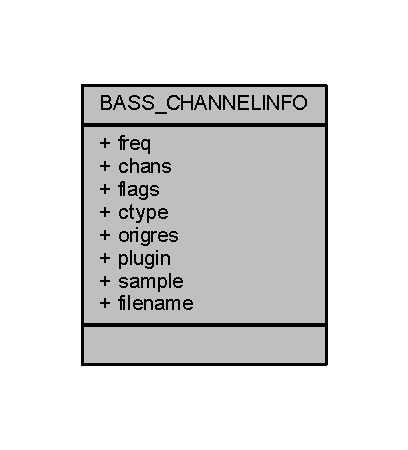
\includegraphics[width=196pt]{struct_b_a_s_s___c_h_a_n_n_e_l_i_n_f_o__coll__graph}
\end{center}
\end{figure}
\subsection*{Public Attributes}
\begin{DoxyCompactItemize}
\item 
\hypertarget{struct_b_a_s_s___c_h_a_n_n_e_l_i_n_f_o_ad1b77f57519254df9076321422ae8088_ad1b77f57519254df9076321422ae8088}{D\-W\-O\-R\-D {\bfseries freq}}\label{struct_b_a_s_s___c_h_a_n_n_e_l_i_n_f_o_ad1b77f57519254df9076321422ae8088_ad1b77f57519254df9076321422ae8088}

\item 
\hypertarget{struct_b_a_s_s___c_h_a_n_n_e_l_i_n_f_o_a6ffe1288a34a2379fe29182ccacd4851_a6ffe1288a34a2379fe29182ccacd4851}{D\-W\-O\-R\-D {\bfseries chans}}\label{struct_b_a_s_s___c_h_a_n_n_e_l_i_n_f_o_a6ffe1288a34a2379fe29182ccacd4851_a6ffe1288a34a2379fe29182ccacd4851}

\item 
\hypertarget{struct_b_a_s_s___c_h_a_n_n_e_l_i_n_f_o_a8af64f94d3e478251a26927f2a4cc181_a8af64f94d3e478251a26927f2a4cc181}{D\-W\-O\-R\-D {\bfseries flags}}\label{struct_b_a_s_s___c_h_a_n_n_e_l_i_n_f_o_a8af64f94d3e478251a26927f2a4cc181_a8af64f94d3e478251a26927f2a4cc181}

\item 
\hypertarget{struct_b_a_s_s___c_h_a_n_n_e_l_i_n_f_o_a8485903de8da5ea87f18af4fead8b109_a8485903de8da5ea87f18af4fead8b109}{D\-W\-O\-R\-D {\bfseries ctype}}\label{struct_b_a_s_s___c_h_a_n_n_e_l_i_n_f_o_a8485903de8da5ea87f18af4fead8b109_a8485903de8da5ea87f18af4fead8b109}

\item 
\hypertarget{struct_b_a_s_s___c_h_a_n_n_e_l_i_n_f_o_a65dafe34621563b319749edff82d824c_a65dafe34621563b319749edff82d824c}{D\-W\-O\-R\-D {\bfseries origres}}\label{struct_b_a_s_s___c_h_a_n_n_e_l_i_n_f_o_a65dafe34621563b319749edff82d824c_a65dafe34621563b319749edff82d824c}

\item 
\hypertarget{struct_b_a_s_s___c_h_a_n_n_e_l_i_n_f_o_a13d3801ae12e966bf36bdf7cf147fd40_a13d3801ae12e966bf36bdf7cf147fd40}{H\-P\-L\-U\-G\-I\-N {\bfseries plugin}}\label{struct_b_a_s_s___c_h_a_n_n_e_l_i_n_f_o_a13d3801ae12e966bf36bdf7cf147fd40_a13d3801ae12e966bf36bdf7cf147fd40}

\item 
\hypertarget{struct_b_a_s_s___c_h_a_n_n_e_l_i_n_f_o_ae2314c04cfb2a04031df1a34d9eb898e_ae2314c04cfb2a04031df1a34d9eb898e}{H\-S\-A\-M\-P\-L\-E {\bfseries sample}}\label{struct_b_a_s_s___c_h_a_n_n_e_l_i_n_f_o_ae2314c04cfb2a04031df1a34d9eb898e_ae2314c04cfb2a04031df1a34d9eb898e}

\item 
\hypertarget{struct_b_a_s_s___c_h_a_n_n_e_l_i_n_f_o_a2e6e5462703ffb79eb85e06e2dc7e62e_a2e6e5462703ffb79eb85e06e2dc7e62e}{const char $\ast$ {\bfseries filename}}\label{struct_b_a_s_s___c_h_a_n_n_e_l_i_n_f_o_a2e6e5462703ffb79eb85e06e2dc7e62e_a2e6e5462703ffb79eb85e06e2dc7e62e}

\end{DoxyCompactItemize}


\subsection{Detailed Description}


Definition at line 316 of file bass.\-h.



The documentation for this struct was generated from the following files\-:\begin{DoxyCompactItemize}
\item 
D\-A\-W\-Components/bass.\-h\item 
M\-S\-Master\-Cmp/bass.\-h\end{DoxyCompactItemize}

\hypertarget{struct_b_a_s_s___d_e_v_i_c_e_i_n_f_o}{\section{B\-A\-S\-S\-\_\-\-D\-E\-V\-I\-C\-E\-I\-N\-F\-O Struct Reference}
\label{struct_b_a_s_s___d_e_v_i_c_e_i_n_f_o}\index{B\-A\-S\-S\-\_\-\-D\-E\-V\-I\-C\-E\-I\-N\-F\-O@{B\-A\-S\-S\-\_\-\-D\-E\-V\-I\-C\-E\-I\-N\-F\-O}}
}


Collaboration diagram for B\-A\-S\-S\-\_\-\-D\-E\-V\-I\-C\-E\-I\-N\-F\-O\-:\nopagebreak
\begin{figure}[H]
\begin{center}
\leavevmode
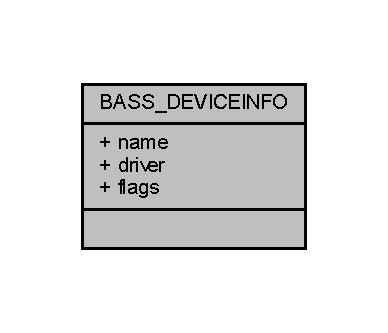
\includegraphics[width=186pt]{struct_b_a_s_s___d_e_v_i_c_e_i_n_f_o__coll__graph}
\end{center}
\end{figure}
\subsection*{Public Attributes}
\begin{DoxyCompactItemize}
\item 
\hypertarget{struct_b_a_s_s___d_e_v_i_c_e_i_n_f_o_a60c99441ee0628febb504c9665bf0f65_a60c99441ee0628febb504c9665bf0f65}{const char $\ast$ {\bfseries name}}\label{struct_b_a_s_s___d_e_v_i_c_e_i_n_f_o_a60c99441ee0628febb504c9665bf0f65_a60c99441ee0628febb504c9665bf0f65}

\item 
\hypertarget{struct_b_a_s_s___d_e_v_i_c_e_i_n_f_o_a9fca2b47e2294e7adad36cecd7e3d7ca_a9fca2b47e2294e7adad36cecd7e3d7ca}{const char $\ast$ {\bfseries driver}}\label{struct_b_a_s_s___d_e_v_i_c_e_i_n_f_o_a9fca2b47e2294e7adad36cecd7e3d7ca_a9fca2b47e2294e7adad36cecd7e3d7ca}

\item 
\hypertarget{struct_b_a_s_s___d_e_v_i_c_e_i_n_f_o_ae5d2db8d3570744a4b24e41dfa62554b_ae5d2db8d3570744a4b24e41dfa62554b}{D\-W\-O\-R\-D {\bfseries flags}}\label{struct_b_a_s_s___d_e_v_i_c_e_i_n_f_o_ae5d2db8d3570744a4b24e41dfa62554b_ae5d2db8d3570744a4b24e41dfa62554b}

\end{DoxyCompactItemize}


\subsection{Detailed Description}


Definition at line 151 of file bass.\-h.



The documentation for this struct was generated from the following files\-:\begin{DoxyCompactItemize}
\item 
D\-A\-W\-Components/bass.\-h\item 
M\-S\-Master\-Cmp/bass.\-h\end{DoxyCompactItemize}

\hypertarget{struct_b_a_s_s___d_x8___c_h_o_r_u_s}{\section{B\-A\-S\-S\-\_\-\-D\-X8\-\_\-\-C\-H\-O\-R\-U\-S Struct Reference}
\label{struct_b_a_s_s___d_x8___c_h_o_r_u_s}\index{B\-A\-S\-S\-\_\-\-D\-X8\-\_\-\-C\-H\-O\-R\-U\-S@{B\-A\-S\-S\-\_\-\-D\-X8\-\_\-\-C\-H\-O\-R\-U\-S}}
}


Collaboration diagram for B\-A\-S\-S\-\_\-\-D\-X8\-\_\-\-C\-H\-O\-R\-U\-S\-:\nopagebreak
\begin{figure}[H]
\begin{center}
\leavevmode
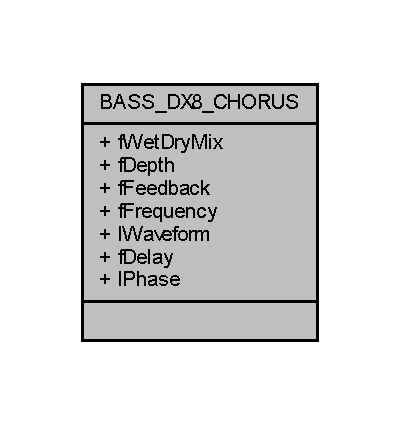
\includegraphics[width=192pt]{struct_b_a_s_s___d_x8___c_h_o_r_u_s__coll__graph}
\end{center}
\end{figure}
\subsection*{Public Attributes}
\begin{DoxyCompactItemize}
\item 
\hypertarget{struct_b_a_s_s___d_x8___c_h_o_r_u_s_ade39ce1bf6ab4e1e4ae192491cf61dd9_ade39ce1bf6ab4e1e4ae192491cf61dd9}{float {\bfseries f\-Wet\-Dry\-Mix}}\label{struct_b_a_s_s___d_x8___c_h_o_r_u_s_ade39ce1bf6ab4e1e4ae192491cf61dd9_ade39ce1bf6ab4e1e4ae192491cf61dd9}

\item 
\hypertarget{struct_b_a_s_s___d_x8___c_h_o_r_u_s_a9255f6285c268622c30999d684e428f5_a9255f6285c268622c30999d684e428f5}{float {\bfseries f\-Depth}}\label{struct_b_a_s_s___d_x8___c_h_o_r_u_s_a9255f6285c268622c30999d684e428f5_a9255f6285c268622c30999d684e428f5}

\item 
\hypertarget{struct_b_a_s_s___d_x8___c_h_o_r_u_s_a3bbcdaa3f0e076111a62e6d9d10b77a8_a3bbcdaa3f0e076111a62e6d9d10b77a8}{float {\bfseries f\-Feedback}}\label{struct_b_a_s_s___d_x8___c_h_o_r_u_s_a3bbcdaa3f0e076111a62e6d9d10b77a8_a3bbcdaa3f0e076111a62e6d9d10b77a8}

\item 
\hypertarget{struct_b_a_s_s___d_x8___c_h_o_r_u_s_a6c28b947dcc6053c08694699625a705f_a6c28b947dcc6053c08694699625a705f}{float {\bfseries f\-Frequency}}\label{struct_b_a_s_s___d_x8___c_h_o_r_u_s_a6c28b947dcc6053c08694699625a705f_a6c28b947dcc6053c08694699625a705f}

\item 
\hypertarget{struct_b_a_s_s___d_x8___c_h_o_r_u_s_ada4ac1a08de4b20c7344d6a28d04a755_ada4ac1a08de4b20c7344d6a28d04a755}{D\-W\-O\-R\-D {\bfseries l\-Waveform}}\label{struct_b_a_s_s___d_x8___c_h_o_r_u_s_ada4ac1a08de4b20c7344d6a28d04a755_ada4ac1a08de4b20c7344d6a28d04a755}

\item 
\hypertarget{struct_b_a_s_s___d_x8___c_h_o_r_u_s_a009967698b28066520e72e3db35a57b3_a009967698b28066520e72e3db35a57b3}{float {\bfseries f\-Delay}}\label{struct_b_a_s_s___d_x8___c_h_o_r_u_s_a009967698b28066520e72e3db35a57b3_a009967698b28066520e72e3db35a57b3}

\item 
\hypertarget{struct_b_a_s_s___d_x8___c_h_o_r_u_s_a98b93f86df1f31303a62c5942ebe3c0e_a98b93f86df1f31303a62c5942ebe3c0e}{D\-W\-O\-R\-D {\bfseries l\-Phase}}\label{struct_b_a_s_s___d_x8___c_h_o_r_u_s_a98b93f86df1f31303a62c5942ebe3c0e_a98b93f86df1f31303a62c5942ebe3c0e}

\end{DoxyCompactItemize}


\subsection{Detailed Description}


Definition at line 754 of file bass.\-h.



The documentation for this struct was generated from the following files\-:\begin{DoxyCompactItemize}
\item 
D\-A\-W\-Components/bass.\-h\item 
M\-S\-Master\-Cmp/bass.\-h\end{DoxyCompactItemize}

\hypertarget{struct_b_a_s_s___d_x8___c_o_m_p_r_e_s_s_o_r}{\section{B\-A\-S\-S\-\_\-\-D\-X8\-\_\-\-C\-O\-M\-P\-R\-E\-S\-S\-O\-R Struct Reference}
\label{struct_b_a_s_s___d_x8___c_o_m_p_r_e_s_s_o_r}\index{B\-A\-S\-S\-\_\-\-D\-X8\-\_\-\-C\-O\-M\-P\-R\-E\-S\-S\-O\-R@{B\-A\-S\-S\-\_\-\-D\-X8\-\_\-\-C\-O\-M\-P\-R\-E\-S\-S\-O\-R}}
}


Collaboration diagram for B\-A\-S\-S\-\_\-\-D\-X8\-\_\-\-C\-O\-M\-P\-R\-E\-S\-S\-O\-R\-:\nopagebreak
\begin{figure}[H]
\begin{center}
\leavevmode
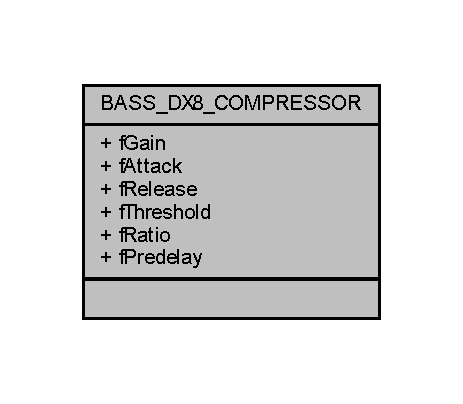
\includegraphics[width=222pt]{struct_b_a_s_s___d_x8___c_o_m_p_r_e_s_s_o_r__coll__graph}
\end{center}
\end{figure}
\subsection*{Public Attributes}
\begin{DoxyCompactItemize}
\item 
\hypertarget{struct_b_a_s_s___d_x8___c_o_m_p_r_e_s_s_o_r_a9d35e7c7ad2df73b081f31ceee1defcc_a9d35e7c7ad2df73b081f31ceee1defcc}{float {\bfseries f\-Gain}}\label{struct_b_a_s_s___d_x8___c_o_m_p_r_e_s_s_o_r_a9d35e7c7ad2df73b081f31ceee1defcc_a9d35e7c7ad2df73b081f31ceee1defcc}

\item 
\hypertarget{struct_b_a_s_s___d_x8___c_o_m_p_r_e_s_s_o_r_a7ad66e4cd902035feff1050abeaf7f35_a7ad66e4cd902035feff1050abeaf7f35}{float {\bfseries f\-Attack}}\label{struct_b_a_s_s___d_x8___c_o_m_p_r_e_s_s_o_r_a7ad66e4cd902035feff1050abeaf7f35_a7ad66e4cd902035feff1050abeaf7f35}

\item 
\hypertarget{struct_b_a_s_s___d_x8___c_o_m_p_r_e_s_s_o_r_a342f2aac54617c7cedb1cef24e504859_a342f2aac54617c7cedb1cef24e504859}{float {\bfseries f\-Release}}\label{struct_b_a_s_s___d_x8___c_o_m_p_r_e_s_s_o_r_a342f2aac54617c7cedb1cef24e504859_a342f2aac54617c7cedb1cef24e504859}

\item 
\hypertarget{struct_b_a_s_s___d_x8___c_o_m_p_r_e_s_s_o_r_a16e3551549e24df55d0f97cb7d67f048_a16e3551549e24df55d0f97cb7d67f048}{float {\bfseries f\-Threshold}}\label{struct_b_a_s_s___d_x8___c_o_m_p_r_e_s_s_o_r_a16e3551549e24df55d0f97cb7d67f048_a16e3551549e24df55d0f97cb7d67f048}

\item 
\hypertarget{struct_b_a_s_s___d_x8___c_o_m_p_r_e_s_s_o_r_adb827cf9d2693779c096cf22761ace59_adb827cf9d2693779c096cf22761ace59}{float {\bfseries f\-Ratio}}\label{struct_b_a_s_s___d_x8___c_o_m_p_r_e_s_s_o_r_adb827cf9d2693779c096cf22761ace59_adb827cf9d2693779c096cf22761ace59}

\item 
\hypertarget{struct_b_a_s_s___d_x8___c_o_m_p_r_e_s_s_o_r_adeacc7ea3f0433fc478b91943a0a695d_adeacc7ea3f0433fc478b91943a0a695d}{float {\bfseries f\-Predelay}}\label{struct_b_a_s_s___d_x8___c_o_m_p_r_e_s_s_o_r_adeacc7ea3f0433fc478b91943a0a695d_adeacc7ea3f0433fc478b91943a0a695d}

\end{DoxyCompactItemize}


\subsection{Detailed Description}


Definition at line 764 of file bass.\-h.



The documentation for this struct was generated from the following files\-:\begin{DoxyCompactItemize}
\item 
D\-A\-W\-Components/bass.\-h\item 
M\-S\-Master\-Cmp/bass.\-h\end{DoxyCompactItemize}

\hypertarget{struct_b_a_s_s___d_x8___d_i_s_t_o_r_t_i_o_n}{\section{B\-A\-S\-S\-\_\-\-D\-X8\-\_\-\-D\-I\-S\-T\-O\-R\-T\-I\-O\-N Struct Reference}
\label{struct_b_a_s_s___d_x8___d_i_s_t_o_r_t_i_o_n}\index{B\-A\-S\-S\-\_\-\-D\-X8\-\_\-\-D\-I\-S\-T\-O\-R\-T\-I\-O\-N@{B\-A\-S\-S\-\_\-\-D\-X8\-\_\-\-D\-I\-S\-T\-O\-R\-T\-I\-O\-N}}
}


Collaboration diagram for B\-A\-S\-S\-\_\-\-D\-X8\-\_\-\-D\-I\-S\-T\-O\-R\-T\-I\-O\-N\-:\nopagebreak
\begin{figure}[H]
\begin{center}
\leavevmode
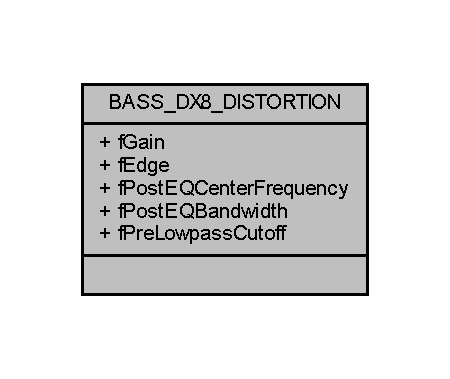
\includegraphics[width=216pt]{struct_b_a_s_s___d_x8___d_i_s_t_o_r_t_i_o_n__coll__graph}
\end{center}
\end{figure}
\subsection*{Public Attributes}
\begin{DoxyCompactItemize}
\item 
\hypertarget{struct_b_a_s_s___d_x8___d_i_s_t_o_r_t_i_o_n_aae2a552fff6dec886b79c64c3c985890_aae2a552fff6dec886b79c64c3c985890}{float {\bfseries f\-Gain}}\label{struct_b_a_s_s___d_x8___d_i_s_t_o_r_t_i_o_n_aae2a552fff6dec886b79c64c3c985890_aae2a552fff6dec886b79c64c3c985890}

\item 
\hypertarget{struct_b_a_s_s___d_x8___d_i_s_t_o_r_t_i_o_n_a277a36a502bed47facd8be9fe06cfb0e_a277a36a502bed47facd8be9fe06cfb0e}{float {\bfseries f\-Edge}}\label{struct_b_a_s_s___d_x8___d_i_s_t_o_r_t_i_o_n_a277a36a502bed47facd8be9fe06cfb0e_a277a36a502bed47facd8be9fe06cfb0e}

\item 
\hypertarget{struct_b_a_s_s___d_x8___d_i_s_t_o_r_t_i_o_n_a90e66d9e0cfc132efa0e68429c5cf81d_a90e66d9e0cfc132efa0e68429c5cf81d}{float {\bfseries f\-Post\-E\-Q\-Center\-Frequency}}\label{struct_b_a_s_s___d_x8___d_i_s_t_o_r_t_i_o_n_a90e66d9e0cfc132efa0e68429c5cf81d_a90e66d9e0cfc132efa0e68429c5cf81d}

\item 
\hypertarget{struct_b_a_s_s___d_x8___d_i_s_t_o_r_t_i_o_n_a0825b5f7724ac6c4c9de9d71c4a48d0b_a0825b5f7724ac6c4c9de9d71c4a48d0b}{float {\bfseries f\-Post\-E\-Q\-Bandwidth}}\label{struct_b_a_s_s___d_x8___d_i_s_t_o_r_t_i_o_n_a0825b5f7724ac6c4c9de9d71c4a48d0b_a0825b5f7724ac6c4c9de9d71c4a48d0b}

\item 
\hypertarget{struct_b_a_s_s___d_x8___d_i_s_t_o_r_t_i_o_n_a1397454ba65a389b7b2a41bb93d10290_a1397454ba65a389b7b2a41bb93d10290}{float {\bfseries f\-Pre\-Lowpass\-Cutoff}}\label{struct_b_a_s_s___d_x8___d_i_s_t_o_r_t_i_o_n_a1397454ba65a389b7b2a41bb93d10290_a1397454ba65a389b7b2a41bb93d10290}

\end{DoxyCompactItemize}


\subsection{Detailed Description}


Definition at line 773 of file bass.\-h.



The documentation for this struct was generated from the following files\-:\begin{DoxyCompactItemize}
\item 
D\-A\-W\-Components/bass.\-h\item 
M\-S\-Master\-Cmp/bass.\-h\end{DoxyCompactItemize}

\hypertarget{struct_b_a_s_s___d_x8___e_c_h_o}{\section{B\-A\-S\-S\-\_\-\-D\-X8\-\_\-\-E\-C\-H\-O Struct Reference}
\label{struct_b_a_s_s___d_x8___e_c_h_o}\index{B\-A\-S\-S\-\_\-\-D\-X8\-\_\-\-E\-C\-H\-O@{B\-A\-S\-S\-\_\-\-D\-X8\-\_\-\-E\-C\-H\-O}}
}


Collaboration diagram for B\-A\-S\-S\-\_\-\-D\-X8\-\_\-\-E\-C\-H\-O\-:\nopagebreak
\begin{figure}[H]
\begin{center}
\leavevmode
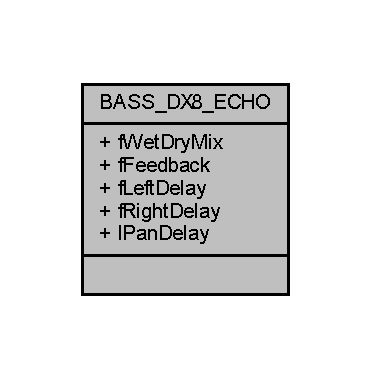
\includegraphics[width=178pt]{struct_b_a_s_s___d_x8___e_c_h_o__coll__graph}
\end{center}
\end{figure}
\subsection*{Public Attributes}
\begin{DoxyCompactItemize}
\item 
\hypertarget{struct_b_a_s_s___d_x8___e_c_h_o_a6c2c28866ef373a669f059f335b6e0f6_a6c2c28866ef373a669f059f335b6e0f6}{float {\bfseries f\-Wet\-Dry\-Mix}}\label{struct_b_a_s_s___d_x8___e_c_h_o_a6c2c28866ef373a669f059f335b6e0f6_a6c2c28866ef373a669f059f335b6e0f6}

\item 
\hypertarget{struct_b_a_s_s___d_x8___e_c_h_o_af0b5c7c7657e2c96594f328f4e864949_af0b5c7c7657e2c96594f328f4e864949}{float {\bfseries f\-Feedback}}\label{struct_b_a_s_s___d_x8___e_c_h_o_af0b5c7c7657e2c96594f328f4e864949_af0b5c7c7657e2c96594f328f4e864949}

\item 
\hypertarget{struct_b_a_s_s___d_x8___e_c_h_o_a191fa91199c5fe5577e01f245cc9eee9_a191fa91199c5fe5577e01f245cc9eee9}{float {\bfseries f\-Left\-Delay}}\label{struct_b_a_s_s___d_x8___e_c_h_o_a191fa91199c5fe5577e01f245cc9eee9_a191fa91199c5fe5577e01f245cc9eee9}

\item 
\hypertarget{struct_b_a_s_s___d_x8___e_c_h_o_a75637c3dcdc3336ff8b6a5dd119af276_a75637c3dcdc3336ff8b6a5dd119af276}{float {\bfseries f\-Right\-Delay}}\label{struct_b_a_s_s___d_x8___e_c_h_o_a75637c3dcdc3336ff8b6a5dd119af276_a75637c3dcdc3336ff8b6a5dd119af276}

\item 
\hypertarget{struct_b_a_s_s___d_x8___e_c_h_o_a60032ed3f9846743ae53468309006a39_a60032ed3f9846743ae53468309006a39}{B\-O\-O\-L {\bfseries l\-Pan\-Delay}}\label{struct_b_a_s_s___d_x8___e_c_h_o_a60032ed3f9846743ae53468309006a39_a60032ed3f9846743ae53468309006a39}

\end{DoxyCompactItemize}


\subsection{Detailed Description}


Definition at line 781 of file bass.\-h.



The documentation for this struct was generated from the following files\-:\begin{DoxyCompactItemize}
\item 
D\-A\-W\-Components/bass.\-h\item 
M\-S\-Master\-Cmp/bass.\-h\end{DoxyCompactItemize}

\hypertarget{struct_b_a_s_s___d_x8___f_l_a_n_g_e_r}{\section{B\-A\-S\-S\-\_\-\-D\-X8\-\_\-\-F\-L\-A\-N\-G\-E\-R Struct Reference}
\label{struct_b_a_s_s___d_x8___f_l_a_n_g_e_r}\index{B\-A\-S\-S\-\_\-\-D\-X8\-\_\-\-F\-L\-A\-N\-G\-E\-R@{B\-A\-S\-S\-\_\-\-D\-X8\-\_\-\-F\-L\-A\-N\-G\-E\-R}}
}


Collaboration diagram for B\-A\-S\-S\-\_\-\-D\-X8\-\_\-\-F\-L\-A\-N\-G\-E\-R\-:\nopagebreak
\begin{figure}[H]
\begin{center}
\leavevmode
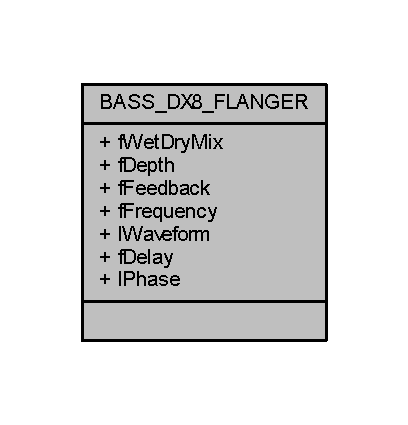
\includegraphics[width=196pt]{struct_b_a_s_s___d_x8___f_l_a_n_g_e_r__coll__graph}
\end{center}
\end{figure}
\subsection*{Public Attributes}
\begin{DoxyCompactItemize}
\item 
\hypertarget{struct_b_a_s_s___d_x8___f_l_a_n_g_e_r_ac538b83d3967c7f5658f05a020f86b1b_ac538b83d3967c7f5658f05a020f86b1b}{float {\bfseries f\-Wet\-Dry\-Mix}}\label{struct_b_a_s_s___d_x8___f_l_a_n_g_e_r_ac538b83d3967c7f5658f05a020f86b1b_ac538b83d3967c7f5658f05a020f86b1b}

\item 
\hypertarget{struct_b_a_s_s___d_x8___f_l_a_n_g_e_r_ad3e6b0734a3eca90563e76d660b41326_ad3e6b0734a3eca90563e76d660b41326}{float {\bfseries f\-Depth}}\label{struct_b_a_s_s___d_x8___f_l_a_n_g_e_r_ad3e6b0734a3eca90563e76d660b41326_ad3e6b0734a3eca90563e76d660b41326}

\item 
\hypertarget{struct_b_a_s_s___d_x8___f_l_a_n_g_e_r_ae28f1dfe21710942e12599ccc6e48ca7_ae28f1dfe21710942e12599ccc6e48ca7}{float {\bfseries f\-Feedback}}\label{struct_b_a_s_s___d_x8___f_l_a_n_g_e_r_ae28f1dfe21710942e12599ccc6e48ca7_ae28f1dfe21710942e12599ccc6e48ca7}

\item 
\hypertarget{struct_b_a_s_s___d_x8___f_l_a_n_g_e_r_ab0bb5ca242d239183c4caa369b7575e7_ab0bb5ca242d239183c4caa369b7575e7}{float {\bfseries f\-Frequency}}\label{struct_b_a_s_s___d_x8___f_l_a_n_g_e_r_ab0bb5ca242d239183c4caa369b7575e7_ab0bb5ca242d239183c4caa369b7575e7}

\item 
\hypertarget{struct_b_a_s_s___d_x8___f_l_a_n_g_e_r_ae05f4fd19f4938bea9b178077f1c6ac5_ae05f4fd19f4938bea9b178077f1c6ac5}{D\-W\-O\-R\-D {\bfseries l\-Waveform}}\label{struct_b_a_s_s___d_x8___f_l_a_n_g_e_r_ae05f4fd19f4938bea9b178077f1c6ac5_ae05f4fd19f4938bea9b178077f1c6ac5}

\item 
\hypertarget{struct_b_a_s_s___d_x8___f_l_a_n_g_e_r_a912410d445465d67601775f4cccdee4e_a912410d445465d67601775f4cccdee4e}{float {\bfseries f\-Delay}}\label{struct_b_a_s_s___d_x8___f_l_a_n_g_e_r_a912410d445465d67601775f4cccdee4e_a912410d445465d67601775f4cccdee4e}

\item 
\hypertarget{struct_b_a_s_s___d_x8___f_l_a_n_g_e_r_a2dd3286e5ffc91673f0f1594ad4d2b8a_a2dd3286e5ffc91673f0f1594ad4d2b8a}{D\-W\-O\-R\-D {\bfseries l\-Phase}}\label{struct_b_a_s_s___d_x8___f_l_a_n_g_e_r_a2dd3286e5ffc91673f0f1594ad4d2b8a_a2dd3286e5ffc91673f0f1594ad4d2b8a}

\end{DoxyCompactItemize}


\subsection{Detailed Description}


Definition at line 789 of file bass.\-h.



The documentation for this struct was generated from the following files\-:\begin{DoxyCompactItemize}
\item 
D\-A\-W\-Components/bass.\-h\item 
M\-S\-Master\-Cmp/bass.\-h\end{DoxyCompactItemize}

\hypertarget{struct_b_a_s_s___d_x8___g_a_r_g_l_e}{\section{B\-A\-S\-S\-\_\-\-D\-X8\-\_\-\-G\-A\-R\-G\-L\-E Struct Reference}
\label{struct_b_a_s_s___d_x8___g_a_r_g_l_e}\index{B\-A\-S\-S\-\_\-\-D\-X8\-\_\-\-G\-A\-R\-G\-L\-E@{B\-A\-S\-S\-\_\-\-D\-X8\-\_\-\-G\-A\-R\-G\-L\-E}}
}


Collaboration diagram for B\-A\-S\-S\-\_\-\-D\-X8\-\_\-\-G\-A\-R\-G\-L\-E\-:\nopagebreak
\begin{figure}[H]
\begin{center}
\leavevmode
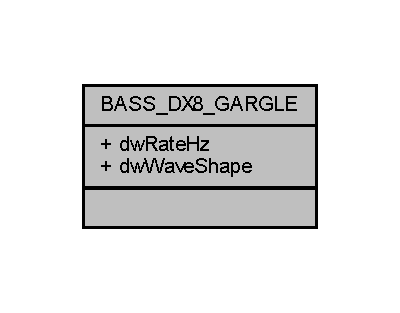
\includegraphics[width=192pt]{struct_b_a_s_s___d_x8___g_a_r_g_l_e__coll__graph}
\end{center}
\end{figure}
\subsection*{Public Attributes}
\begin{DoxyCompactItemize}
\item 
\hypertarget{struct_b_a_s_s___d_x8___g_a_r_g_l_e_a0338a456e4a61784c095203642b3e801_a0338a456e4a61784c095203642b3e801}{D\-W\-O\-R\-D {\bfseries dw\-Rate\-Hz}}\label{struct_b_a_s_s___d_x8___g_a_r_g_l_e_a0338a456e4a61784c095203642b3e801_a0338a456e4a61784c095203642b3e801}

\item 
\hypertarget{struct_b_a_s_s___d_x8___g_a_r_g_l_e_aca685edf6d4938d62830ce4a834f0e28_aca685edf6d4938d62830ce4a834f0e28}{D\-W\-O\-R\-D {\bfseries dw\-Wave\-Shape}}\label{struct_b_a_s_s___d_x8___g_a_r_g_l_e_aca685edf6d4938d62830ce4a834f0e28_aca685edf6d4938d62830ce4a834f0e28}

\end{DoxyCompactItemize}


\subsection{Detailed Description}


Definition at line 799 of file bass.\-h.



The documentation for this struct was generated from the following files\-:\begin{DoxyCompactItemize}
\item 
D\-A\-W\-Components/bass.\-h\item 
M\-S\-Master\-Cmp/bass.\-h\end{DoxyCompactItemize}

\hypertarget{struct_b_a_s_s___d_x8___i3_d_l2_r_e_v_e_r_b}{\section{B\-A\-S\-S\-\_\-\-D\-X8\-\_\-\-I3\-D\-L2\-R\-E\-V\-E\-R\-B Struct Reference}
\label{struct_b_a_s_s___d_x8___i3_d_l2_r_e_v_e_r_b}\index{B\-A\-S\-S\-\_\-\-D\-X8\-\_\-\-I3\-D\-L2\-R\-E\-V\-E\-R\-B@{B\-A\-S\-S\-\_\-\-D\-X8\-\_\-\-I3\-D\-L2\-R\-E\-V\-E\-R\-B}}
}


Collaboration diagram for B\-A\-S\-S\-\_\-\-D\-X8\-\_\-\-I3\-D\-L2\-R\-E\-V\-E\-R\-B\-:\nopagebreak
\begin{figure}[H]
\begin{center}
\leavevmode
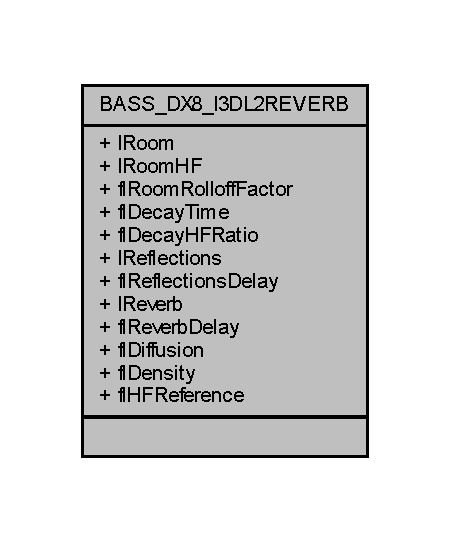
\includegraphics[width=216pt]{struct_b_a_s_s___d_x8___i3_d_l2_r_e_v_e_r_b__coll__graph}
\end{center}
\end{figure}
\subsection*{Public Attributes}
\begin{DoxyCompactItemize}
\item 
\hypertarget{struct_b_a_s_s___d_x8___i3_d_l2_r_e_v_e_r_b_a520686858323f3210f4c36d6a9cb510c_a520686858323f3210f4c36d6a9cb510c}{int {\bfseries l\-Room}}\label{struct_b_a_s_s___d_x8___i3_d_l2_r_e_v_e_r_b_a520686858323f3210f4c36d6a9cb510c_a520686858323f3210f4c36d6a9cb510c}

\item 
\hypertarget{struct_b_a_s_s___d_x8___i3_d_l2_r_e_v_e_r_b_a808a172f5de62ae509adc6fa2c403537_a808a172f5de62ae509adc6fa2c403537}{int {\bfseries l\-Room\-H\-F}}\label{struct_b_a_s_s___d_x8___i3_d_l2_r_e_v_e_r_b_a808a172f5de62ae509adc6fa2c403537_a808a172f5de62ae509adc6fa2c403537}

\item 
\hypertarget{struct_b_a_s_s___d_x8___i3_d_l2_r_e_v_e_r_b_ac4e7a936bb33324e4f2845ae4a5d7d4c_ac4e7a936bb33324e4f2845ae4a5d7d4c}{float {\bfseries fl\-Room\-Rolloff\-Factor}}\label{struct_b_a_s_s___d_x8___i3_d_l2_r_e_v_e_r_b_ac4e7a936bb33324e4f2845ae4a5d7d4c_ac4e7a936bb33324e4f2845ae4a5d7d4c}

\item 
\hypertarget{struct_b_a_s_s___d_x8___i3_d_l2_r_e_v_e_r_b_a4698afcd5cb82a19422122e048c488a5_a4698afcd5cb82a19422122e048c488a5}{float {\bfseries fl\-Decay\-Time}}\label{struct_b_a_s_s___d_x8___i3_d_l2_r_e_v_e_r_b_a4698afcd5cb82a19422122e048c488a5_a4698afcd5cb82a19422122e048c488a5}

\item 
\hypertarget{struct_b_a_s_s___d_x8___i3_d_l2_r_e_v_e_r_b_a86d473034e7f77d712d0f4c9595956c3_a86d473034e7f77d712d0f4c9595956c3}{float {\bfseries fl\-Decay\-H\-F\-Ratio}}\label{struct_b_a_s_s___d_x8___i3_d_l2_r_e_v_e_r_b_a86d473034e7f77d712d0f4c9595956c3_a86d473034e7f77d712d0f4c9595956c3}

\item 
\hypertarget{struct_b_a_s_s___d_x8___i3_d_l2_r_e_v_e_r_b_a218715f13676217b76c0ffaf4f9a1b1b_a218715f13676217b76c0ffaf4f9a1b1b}{int {\bfseries l\-Reflections}}\label{struct_b_a_s_s___d_x8___i3_d_l2_r_e_v_e_r_b_a218715f13676217b76c0ffaf4f9a1b1b_a218715f13676217b76c0ffaf4f9a1b1b}

\item 
\hypertarget{struct_b_a_s_s___d_x8___i3_d_l2_r_e_v_e_r_b_a2f14853c94f1c1a9cd2c262ec184f0a5_a2f14853c94f1c1a9cd2c262ec184f0a5}{float {\bfseries fl\-Reflections\-Delay}}\label{struct_b_a_s_s___d_x8___i3_d_l2_r_e_v_e_r_b_a2f14853c94f1c1a9cd2c262ec184f0a5_a2f14853c94f1c1a9cd2c262ec184f0a5}

\item 
\hypertarget{struct_b_a_s_s___d_x8___i3_d_l2_r_e_v_e_r_b_abb5ecb3324ef2baf89a705b7ea2e2b11_abb5ecb3324ef2baf89a705b7ea2e2b11}{int {\bfseries l\-Reverb}}\label{struct_b_a_s_s___d_x8___i3_d_l2_r_e_v_e_r_b_abb5ecb3324ef2baf89a705b7ea2e2b11_abb5ecb3324ef2baf89a705b7ea2e2b11}

\item 
\hypertarget{struct_b_a_s_s___d_x8___i3_d_l2_r_e_v_e_r_b_a6b4b4d42d466a042dcce95a9b6ffc75a_a6b4b4d42d466a042dcce95a9b6ffc75a}{float {\bfseries fl\-Reverb\-Delay}}\label{struct_b_a_s_s___d_x8___i3_d_l2_r_e_v_e_r_b_a6b4b4d42d466a042dcce95a9b6ffc75a_a6b4b4d42d466a042dcce95a9b6ffc75a}

\item 
\hypertarget{struct_b_a_s_s___d_x8___i3_d_l2_r_e_v_e_r_b_a68c326cead487bc08eb060ff0492029a_a68c326cead487bc08eb060ff0492029a}{float {\bfseries fl\-Diffusion}}\label{struct_b_a_s_s___d_x8___i3_d_l2_r_e_v_e_r_b_a68c326cead487bc08eb060ff0492029a_a68c326cead487bc08eb060ff0492029a}

\item 
\hypertarget{struct_b_a_s_s___d_x8___i3_d_l2_r_e_v_e_r_b_a74924c051e337eabbe439bea2e4cfb15_a74924c051e337eabbe439bea2e4cfb15}{float {\bfseries fl\-Density}}\label{struct_b_a_s_s___d_x8___i3_d_l2_r_e_v_e_r_b_a74924c051e337eabbe439bea2e4cfb15_a74924c051e337eabbe439bea2e4cfb15}

\item 
\hypertarget{struct_b_a_s_s___d_x8___i3_d_l2_r_e_v_e_r_b_a3074421854b36b937c7d4cb22606fc9d_a3074421854b36b937c7d4cb22606fc9d}{float {\bfseries fl\-H\-F\-Reference}}\label{struct_b_a_s_s___d_x8___i3_d_l2_r_e_v_e_r_b_a3074421854b36b937c7d4cb22606fc9d_a3074421854b36b937c7d4cb22606fc9d}

\end{DoxyCompactItemize}


\subsection{Detailed Description}


Definition at line 804 of file bass.\-h.



The documentation for this struct was generated from the following files\-:\begin{DoxyCompactItemize}
\item 
D\-A\-W\-Components/bass.\-h\item 
M\-S\-Master\-Cmp/bass.\-h\end{DoxyCompactItemize}

\hypertarget{struct_b_a_s_s___d_x8___p_a_r_a_m_e_q}{\section{B\-A\-S\-S\-\_\-\-D\-X8\-\_\-\-P\-A\-R\-A\-M\-E\-Q Struct Reference}
\label{struct_b_a_s_s___d_x8___p_a_r_a_m_e_q}\index{B\-A\-S\-S\-\_\-\-D\-X8\-\_\-\-P\-A\-R\-A\-M\-E\-Q@{B\-A\-S\-S\-\_\-\-D\-X8\-\_\-\-P\-A\-R\-A\-M\-E\-Q}}
}


Collaboration diagram for B\-A\-S\-S\-\_\-\-D\-X8\-\_\-\-P\-A\-R\-A\-M\-E\-Q\-:\nopagebreak
\begin{figure}[H]
\begin{center}
\leavevmode
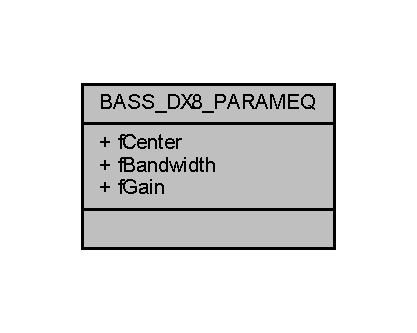
\includegraphics[width=200pt]{struct_b_a_s_s___d_x8___p_a_r_a_m_e_q__coll__graph}
\end{center}
\end{figure}
\subsection*{Public Attributes}
\begin{DoxyCompactItemize}
\item 
\hypertarget{struct_b_a_s_s___d_x8___p_a_r_a_m_e_q_ab0774aabf58f7e8eb28213a710713c4e_ab0774aabf58f7e8eb28213a710713c4e}{float {\bfseries f\-Center}}\label{struct_b_a_s_s___d_x8___p_a_r_a_m_e_q_ab0774aabf58f7e8eb28213a710713c4e_ab0774aabf58f7e8eb28213a710713c4e}

\item 
\hypertarget{struct_b_a_s_s___d_x8___p_a_r_a_m_e_q_a93e4f82cbba760d52f2f3b0703c36b8b_a93e4f82cbba760d52f2f3b0703c36b8b}{float {\bfseries f\-Bandwidth}}\label{struct_b_a_s_s___d_x8___p_a_r_a_m_e_q_a93e4f82cbba760d52f2f3b0703c36b8b_a93e4f82cbba760d52f2f3b0703c36b8b}

\item 
\hypertarget{struct_b_a_s_s___d_x8___p_a_r_a_m_e_q_ab573fd8cee48cc9ce5d0c2264bc0394d_ab573fd8cee48cc9ce5d0c2264bc0394d}{float {\bfseries f\-Gain}}\label{struct_b_a_s_s___d_x8___p_a_r_a_m_e_q_ab573fd8cee48cc9ce5d0c2264bc0394d_ab573fd8cee48cc9ce5d0c2264bc0394d}

\end{DoxyCompactItemize}


\subsection{Detailed Description}


Definition at line 819 of file bass.\-h.



The documentation for this struct was generated from the following files\-:\begin{DoxyCompactItemize}
\item 
D\-A\-W\-Components/bass.\-h\item 
M\-S\-Master\-Cmp/bass.\-h\end{DoxyCompactItemize}

\hypertarget{struct_b_a_s_s___d_x8___r_e_v_e_r_b}{\section{B\-A\-S\-S\-\_\-\-D\-X8\-\_\-\-R\-E\-V\-E\-R\-B Struct Reference}
\label{struct_b_a_s_s___d_x8___r_e_v_e_r_b}\index{B\-A\-S\-S\-\_\-\-D\-X8\-\_\-\-R\-E\-V\-E\-R\-B@{B\-A\-S\-S\-\_\-\-D\-X8\-\_\-\-R\-E\-V\-E\-R\-B}}
}


Collaboration diagram for B\-A\-S\-S\-\_\-\-D\-X8\-\_\-\-R\-E\-V\-E\-R\-B\-:\nopagebreak
\begin{figure}[H]
\begin{center}
\leavevmode
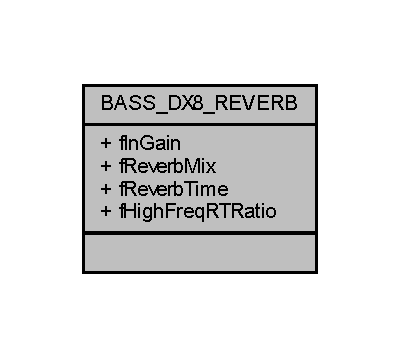
\includegraphics[width=192pt]{struct_b_a_s_s___d_x8___r_e_v_e_r_b__coll__graph}
\end{center}
\end{figure}
\subsection*{Public Attributes}
\begin{DoxyCompactItemize}
\item 
\hypertarget{struct_b_a_s_s___d_x8___r_e_v_e_r_b_a3e6c02bdd61a3fae050c6a7f9318edd6_a3e6c02bdd61a3fae050c6a7f9318edd6}{float {\bfseries f\-In\-Gain}}\label{struct_b_a_s_s___d_x8___r_e_v_e_r_b_a3e6c02bdd61a3fae050c6a7f9318edd6_a3e6c02bdd61a3fae050c6a7f9318edd6}

\item 
\hypertarget{struct_b_a_s_s___d_x8___r_e_v_e_r_b_aaf55c48b1628fde8c6834fa5a223d807_aaf55c48b1628fde8c6834fa5a223d807}{float {\bfseries f\-Reverb\-Mix}}\label{struct_b_a_s_s___d_x8___r_e_v_e_r_b_aaf55c48b1628fde8c6834fa5a223d807_aaf55c48b1628fde8c6834fa5a223d807}

\item 
\hypertarget{struct_b_a_s_s___d_x8___r_e_v_e_r_b_adb97abb30a9a52c71e7a01d0b1c9b597_adb97abb30a9a52c71e7a01d0b1c9b597}{float {\bfseries f\-Reverb\-Time}}\label{struct_b_a_s_s___d_x8___r_e_v_e_r_b_adb97abb30a9a52c71e7a01d0b1c9b597_adb97abb30a9a52c71e7a01d0b1c9b597}

\item 
\hypertarget{struct_b_a_s_s___d_x8___r_e_v_e_r_b_ac19b8eddbad1b31e88ac508ccaa08a2d_ac19b8eddbad1b31e88ac508ccaa08a2d}{float {\bfseries f\-High\-Freq\-R\-T\-Ratio}}\label{struct_b_a_s_s___d_x8___r_e_v_e_r_b_ac19b8eddbad1b31e88ac508ccaa08a2d_ac19b8eddbad1b31e88ac508ccaa08a2d}

\end{DoxyCompactItemize}


\subsection{Detailed Description}


Definition at line 825 of file bass.\-h.



The documentation for this struct was generated from the following files\-:\begin{DoxyCompactItemize}
\item 
D\-A\-W\-Components/bass.\-h\item 
M\-S\-Master\-Cmp/bass.\-h\end{DoxyCompactItemize}

\hypertarget{struct_b_a_s_s___f_i_l_e_p_r_o_c_s}{\section{B\-A\-S\-S\-\_\-\-F\-I\-L\-E\-P\-R\-O\-C\-S Struct Reference}
\label{struct_b_a_s_s___f_i_l_e_p_r_o_c_s}\index{B\-A\-S\-S\-\_\-\-F\-I\-L\-E\-P\-R\-O\-C\-S@{B\-A\-S\-S\-\_\-\-F\-I\-L\-E\-P\-R\-O\-C\-S}}
}


Collaboration diagram for B\-A\-S\-S\-\_\-\-F\-I\-L\-E\-P\-R\-O\-C\-S\-:\nopagebreak
\begin{figure}[H]
\begin{center}
\leavevmode
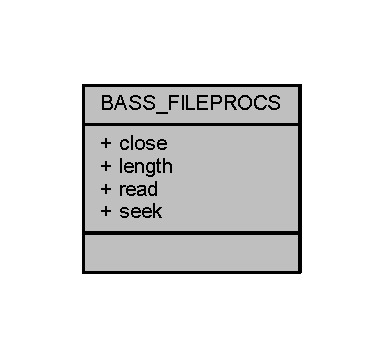
\includegraphics[width=184pt]{struct_b_a_s_s___f_i_l_e_p_r_o_c_s__coll__graph}
\end{center}
\end{figure}
\subsection*{Public Attributes}
\begin{DoxyCompactItemize}
\item 
\hypertarget{struct_b_a_s_s___f_i_l_e_p_r_o_c_s_ad59646dcd884fd17f03f287aa4357f41_ad59646dcd884fd17f03f287aa4357f41}{F\-I\-L\-E\-C\-L\-O\-S\-E\-P\-R\-O\-C $\ast$ {\bfseries close}}\label{struct_b_a_s_s___f_i_l_e_p_r_o_c_s_ad59646dcd884fd17f03f287aa4357f41_ad59646dcd884fd17f03f287aa4357f41}

\item 
\hypertarget{struct_b_a_s_s___f_i_l_e_p_r_o_c_s_ac1f07354d8eac94a95391c6f5c12529f_ac1f07354d8eac94a95391c6f5c12529f}{F\-I\-L\-E\-L\-E\-N\-P\-R\-O\-C $\ast$ {\bfseries length}}\label{struct_b_a_s_s___f_i_l_e_p_r_o_c_s_ac1f07354d8eac94a95391c6f5c12529f_ac1f07354d8eac94a95391c6f5c12529f}

\item 
\hypertarget{struct_b_a_s_s___f_i_l_e_p_r_o_c_s_a8492fd4a894c34f80c7417c23bf7306d_a8492fd4a894c34f80c7417c23bf7306d}{F\-I\-L\-E\-R\-E\-A\-D\-P\-R\-O\-C $\ast$ {\bfseries read}}\label{struct_b_a_s_s___f_i_l_e_p_r_o_c_s_a8492fd4a894c34f80c7417c23bf7306d_a8492fd4a894c34f80c7417c23bf7306d}

\item 
\hypertarget{struct_b_a_s_s___f_i_l_e_p_r_o_c_s_a1a84987b5f65ebfc09ab728a55922d72_a1a84987b5f65ebfc09ab728a55922d72}{F\-I\-L\-E\-S\-E\-E\-K\-P\-R\-O\-C $\ast$ {\bfseries seek}}\label{struct_b_a_s_s___f_i_l_e_p_r_o_c_s_a1a84987b5f65ebfc09ab728a55922d72_a1a84987b5f65ebfc09ab728a55922d72}

\end{DoxyCompactItemize}


\subsection{Detailed Description}


Definition at line 475 of file bass.\-h.



The documentation for this struct was generated from the following files\-:\begin{DoxyCompactItemize}
\item 
D\-A\-W\-Components/bass.\-h\item 
M\-S\-Master\-Cmp/bass.\-h\end{DoxyCompactItemize}

\hypertarget{struct_b_a_s_s___i_n_f_o}{\section{B\-A\-S\-S\-\_\-\-I\-N\-F\-O Struct Reference}
\label{struct_b_a_s_s___i_n_f_o}\index{B\-A\-S\-S\-\_\-\-I\-N\-F\-O@{B\-A\-S\-S\-\_\-\-I\-N\-F\-O}}
}


Collaboration diagram for B\-A\-S\-S\-\_\-\-I\-N\-F\-O\-:\nopagebreak
\begin{figure}[H]
\begin{center}
\leavevmode
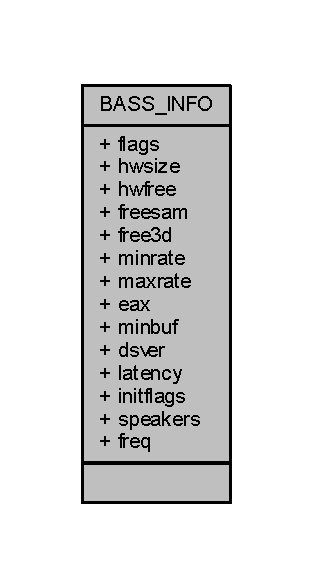
\includegraphics[width=150pt]{struct_b_a_s_s___i_n_f_o__coll__graph}
\end{center}
\end{figure}
\subsection*{Public Attributes}
\begin{DoxyCompactItemize}
\item 
\hypertarget{struct_b_a_s_s___i_n_f_o_acc4ee63d143d96b60e96fe55ad66d151_acc4ee63d143d96b60e96fe55ad66d151}{D\-W\-O\-R\-D {\bfseries flags}}\label{struct_b_a_s_s___i_n_f_o_acc4ee63d143d96b60e96fe55ad66d151_acc4ee63d143d96b60e96fe55ad66d151}

\item 
\hypertarget{struct_b_a_s_s___i_n_f_o_a41c357da1c1d00b688c237719acb668b_a41c357da1c1d00b688c237719acb668b}{D\-W\-O\-R\-D {\bfseries hwsize}}\label{struct_b_a_s_s___i_n_f_o_a41c357da1c1d00b688c237719acb668b_a41c357da1c1d00b688c237719acb668b}

\item 
\hypertarget{struct_b_a_s_s___i_n_f_o_a2e7b2bdba56ca19846702cc2251dceaf_a2e7b2bdba56ca19846702cc2251dceaf}{D\-W\-O\-R\-D {\bfseries hwfree}}\label{struct_b_a_s_s___i_n_f_o_a2e7b2bdba56ca19846702cc2251dceaf_a2e7b2bdba56ca19846702cc2251dceaf}

\item 
\hypertarget{struct_b_a_s_s___i_n_f_o_a1ec0d1abc45e959efd8324a729108eca_a1ec0d1abc45e959efd8324a729108eca}{D\-W\-O\-R\-D {\bfseries freesam}}\label{struct_b_a_s_s___i_n_f_o_a1ec0d1abc45e959efd8324a729108eca_a1ec0d1abc45e959efd8324a729108eca}

\item 
\hypertarget{struct_b_a_s_s___i_n_f_o_a04951fd8ee77cdf358ae897e64318f51_a04951fd8ee77cdf358ae897e64318f51}{D\-W\-O\-R\-D {\bfseries free3d}}\label{struct_b_a_s_s___i_n_f_o_a04951fd8ee77cdf358ae897e64318f51_a04951fd8ee77cdf358ae897e64318f51}

\item 
\hypertarget{struct_b_a_s_s___i_n_f_o_ae98cb552509ca0cf8a6f034544ad9523_ae98cb552509ca0cf8a6f034544ad9523}{D\-W\-O\-R\-D {\bfseries minrate}}\label{struct_b_a_s_s___i_n_f_o_ae98cb552509ca0cf8a6f034544ad9523_ae98cb552509ca0cf8a6f034544ad9523}

\item 
\hypertarget{struct_b_a_s_s___i_n_f_o_a770602ac32b59b0b563da64276e8110e_a770602ac32b59b0b563da64276e8110e}{D\-W\-O\-R\-D {\bfseries maxrate}}\label{struct_b_a_s_s___i_n_f_o_a770602ac32b59b0b563da64276e8110e_a770602ac32b59b0b563da64276e8110e}

\item 
\hypertarget{struct_b_a_s_s___i_n_f_o_adab4375ade13fe88510db582bd3c919f_adab4375ade13fe88510db582bd3c919f}{B\-O\-O\-L {\bfseries eax}}\label{struct_b_a_s_s___i_n_f_o_adab4375ade13fe88510db582bd3c919f_adab4375ade13fe88510db582bd3c919f}

\item 
\hypertarget{struct_b_a_s_s___i_n_f_o_a855c6df53310491802f018736e81dac4_a855c6df53310491802f018736e81dac4}{D\-W\-O\-R\-D {\bfseries minbuf}}\label{struct_b_a_s_s___i_n_f_o_a855c6df53310491802f018736e81dac4_a855c6df53310491802f018736e81dac4}

\item 
\hypertarget{struct_b_a_s_s___i_n_f_o_af8cabba039215c378dd6fd6ef0bf8e9f_af8cabba039215c378dd6fd6ef0bf8e9f}{D\-W\-O\-R\-D {\bfseries dsver}}\label{struct_b_a_s_s___i_n_f_o_af8cabba039215c378dd6fd6ef0bf8e9f_af8cabba039215c378dd6fd6ef0bf8e9f}

\item 
\hypertarget{struct_b_a_s_s___i_n_f_o_ab54c862f3f10d31df27541c83682c883_ab54c862f3f10d31df27541c83682c883}{D\-W\-O\-R\-D {\bfseries latency}}\label{struct_b_a_s_s___i_n_f_o_ab54c862f3f10d31df27541c83682c883_ab54c862f3f10d31df27541c83682c883}

\item 
\hypertarget{struct_b_a_s_s___i_n_f_o_a7c73adb1a84b1c7b2af2da81694e24da_a7c73adb1a84b1c7b2af2da81694e24da}{D\-W\-O\-R\-D {\bfseries initflags}}\label{struct_b_a_s_s___i_n_f_o_a7c73adb1a84b1c7b2af2da81694e24da_a7c73adb1a84b1c7b2af2da81694e24da}

\item 
\hypertarget{struct_b_a_s_s___i_n_f_o_a5b563d324e9551ab98ce9888c5277f72_a5b563d324e9551ab98ce9888c5277f72}{D\-W\-O\-R\-D {\bfseries speakers}}\label{struct_b_a_s_s___i_n_f_o_a5b563d324e9551ab98ce9888c5277f72_a5b563d324e9551ab98ce9888c5277f72}

\item 
\hypertarget{struct_b_a_s_s___i_n_f_o_a72d42df53abce9b0fd676aa220b377ad_a72d42df53abce9b0fd676aa220b377ad}{D\-W\-O\-R\-D {\bfseries freq}}\label{struct_b_a_s_s___i_n_f_o_a72d42df53abce9b0fd676aa220b377ad_a72d42df53abce9b0fd676aa220b377ad}

\end{DoxyCompactItemize}


\subsection{Detailed Description}


Definition at line 167 of file bass.\-h.



The documentation for this struct was generated from the following files\-:\begin{DoxyCompactItemize}
\item 
D\-A\-W\-Components/bass.\-h\item 
M\-S\-Master\-Cmp/bass.\-h\end{DoxyCompactItemize}

\hypertarget{struct_b_a_s_s___m_i_x_e_r___n_o_d_e}{\section{B\-A\-S\-S\-\_\-\-M\-I\-X\-E\-R\-\_\-\-N\-O\-D\-E Struct Reference}
\label{struct_b_a_s_s___m_i_x_e_r___n_o_d_e}\index{B\-A\-S\-S\-\_\-\-M\-I\-X\-E\-R\-\_\-\-N\-O\-D\-E@{B\-A\-S\-S\-\_\-\-M\-I\-X\-E\-R\-\_\-\-N\-O\-D\-E}}
}


Collaboration diagram for B\-A\-S\-S\-\_\-\-M\-I\-X\-E\-R\-\_\-\-N\-O\-D\-E\-:\nopagebreak
\begin{figure}[H]
\begin{center}
\leavevmode
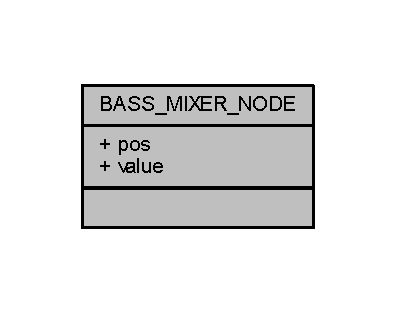
\includegraphics[width=190pt]{struct_b_a_s_s___m_i_x_e_r___n_o_d_e__coll__graph}
\end{center}
\end{figure}
\subsection*{Public Attributes}
\begin{DoxyCompactItemize}
\item 
\hypertarget{struct_b_a_s_s___m_i_x_e_r___n_o_d_e_af4010e38e85d9f9ddadfdd18bd60f7b5_af4010e38e85d9f9ddadfdd18bd60f7b5}{Q\-W\-O\-R\-D {\bfseries pos}}\label{struct_b_a_s_s___m_i_x_e_r___n_o_d_e_af4010e38e85d9f9ddadfdd18bd60f7b5_af4010e38e85d9f9ddadfdd18bd60f7b5}

\item 
\hypertarget{struct_b_a_s_s___m_i_x_e_r___n_o_d_e_a545b3a15ac920fa4a6a63059c5387cc4_a545b3a15ac920fa4a6a63059c5387cc4}{float {\bfseries value}}\label{struct_b_a_s_s___m_i_x_e_r___n_o_d_e_a545b3a15ac920fa4a6a63059c5387cc4_a545b3a15ac920fa4a6a63059c5387cc4}

\end{DoxyCompactItemize}


\subsection{Detailed Description}


Definition at line 48 of file bassmix.\-h.



The documentation for this struct was generated from the following file\-:\begin{DoxyCompactItemize}
\item 
M\-S\-Master\-Cmp/bassmix.\-h\end{DoxyCompactItemize}

\hypertarget{struct_b_a_s_s___p_l_u_g_i_n_f_o_r_m}{\section{B\-A\-S\-S\-\_\-\-P\-L\-U\-G\-I\-N\-F\-O\-R\-M Struct Reference}
\label{struct_b_a_s_s___p_l_u_g_i_n_f_o_r_m}\index{B\-A\-S\-S\-\_\-\-P\-L\-U\-G\-I\-N\-F\-O\-R\-M@{B\-A\-S\-S\-\_\-\-P\-L\-U\-G\-I\-N\-F\-O\-R\-M}}
}


Collaboration diagram for B\-A\-S\-S\-\_\-\-P\-L\-U\-G\-I\-N\-F\-O\-R\-M\-:\nopagebreak
\begin{figure}[H]
\begin{center}
\leavevmode
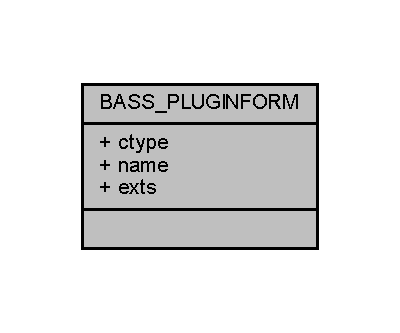
\includegraphics[width=192pt]{struct_b_a_s_s___p_l_u_g_i_n_f_o_r_m__coll__graph}
\end{center}
\end{figure}
\subsection*{Public Attributes}
\begin{DoxyCompactItemize}
\item 
\hypertarget{struct_b_a_s_s___p_l_u_g_i_n_f_o_r_m_a93952bbca5695ff5c9e1bdc8e7271368_a93952bbca5695ff5c9e1bdc8e7271368}{D\-W\-O\-R\-D {\bfseries ctype}}\label{struct_b_a_s_s___p_l_u_g_i_n_f_o_r_m_a93952bbca5695ff5c9e1bdc8e7271368_a93952bbca5695ff5c9e1bdc8e7271368}

\item 
\hypertarget{struct_b_a_s_s___p_l_u_g_i_n_f_o_r_m_a019e8e170022de437a102c9997a15103_a019e8e170022de437a102c9997a15103}{const char $\ast$ {\bfseries name}}\label{struct_b_a_s_s___p_l_u_g_i_n_f_o_r_m_a019e8e170022de437a102c9997a15103_a019e8e170022de437a102c9997a15103}

\item 
\hypertarget{struct_b_a_s_s___p_l_u_g_i_n_f_o_r_m_a9de1247713a7b5fe0ef8d285878e3159_a9de1247713a7b5fe0ef8d285878e3159}{const char $\ast$ {\bfseries exts}}\label{struct_b_a_s_s___p_l_u_g_i_n_f_o_r_m_a9de1247713a7b5fe0ef8d285878e3159_a9de1247713a7b5fe0ef8d285878e3159}

\end{DoxyCompactItemize}


\subsection{Detailed Description}


Definition at line 348 of file bass.\-h.



The documentation for this struct was generated from the following files\-:\begin{DoxyCompactItemize}
\item 
D\-A\-W\-Components/bass.\-h\item 
M\-S\-Master\-Cmp/bass.\-h\end{DoxyCompactItemize}

\hypertarget{struct_b_a_s_s___p_l_u_g_i_n_i_n_f_o}{\section{B\-A\-S\-S\-\_\-\-P\-L\-U\-G\-I\-N\-I\-N\-F\-O Struct Reference}
\label{struct_b_a_s_s___p_l_u_g_i_n_i_n_f_o}\index{B\-A\-S\-S\-\_\-\-P\-L\-U\-G\-I\-N\-I\-N\-F\-O@{B\-A\-S\-S\-\_\-\-P\-L\-U\-G\-I\-N\-I\-N\-F\-O}}
}


Collaboration diagram for B\-A\-S\-S\-\_\-\-P\-L\-U\-G\-I\-N\-I\-N\-F\-O\-:\nopagebreak
\begin{figure}[H]
\begin{center}
\leavevmode
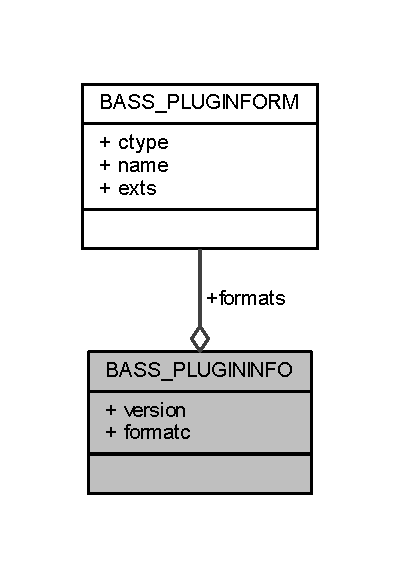
\includegraphics[width=192pt]{struct_b_a_s_s___p_l_u_g_i_n_i_n_f_o__coll__graph}
\end{center}
\end{figure}
\subsection*{Public Attributes}
\begin{DoxyCompactItemize}
\item 
\hypertarget{struct_b_a_s_s___p_l_u_g_i_n_i_n_f_o_a893c8f212060896e986b82487c9710a2_a893c8f212060896e986b82487c9710a2}{D\-W\-O\-R\-D {\bfseries version}}\label{struct_b_a_s_s___p_l_u_g_i_n_i_n_f_o_a893c8f212060896e986b82487c9710a2_a893c8f212060896e986b82487c9710a2}

\item 
\hypertarget{struct_b_a_s_s___p_l_u_g_i_n_i_n_f_o_a45daf6218ce12dd4e8fc01316b9852e9_a45daf6218ce12dd4e8fc01316b9852e9}{D\-W\-O\-R\-D {\bfseries formatc}}\label{struct_b_a_s_s___p_l_u_g_i_n_i_n_f_o_a45daf6218ce12dd4e8fc01316b9852e9_a45daf6218ce12dd4e8fc01316b9852e9}

\item 
\hypertarget{struct_b_a_s_s___p_l_u_g_i_n_i_n_f_o_a1db793e75635c11854a924f4f42c3376_a1db793e75635c11854a924f4f42c3376}{const \hyperlink{struct_b_a_s_s___p_l_u_g_i_n_f_o_r_m}{B\-A\-S\-S\-\_\-\-P\-L\-U\-G\-I\-N\-F\-O\-R\-M} $\ast$ {\bfseries formats}}\label{struct_b_a_s_s___p_l_u_g_i_n_i_n_f_o_a1db793e75635c11854a924f4f42c3376_a1db793e75635c11854a924f4f42c3376}

\end{DoxyCompactItemize}


\subsection{Detailed Description}


Definition at line 359 of file bass.\-h.



The documentation for this struct was generated from the following files\-:\begin{DoxyCompactItemize}
\item 
D\-A\-W\-Components/bass.\-h\item 
M\-S\-Master\-Cmp/bass.\-h\end{DoxyCompactItemize}

\hypertarget{struct_b_a_s_s___r_e_c_o_r_d_i_n_f_o}{\section{B\-A\-S\-S\-\_\-\-R\-E\-C\-O\-R\-D\-I\-N\-F\-O Struct Reference}
\label{struct_b_a_s_s___r_e_c_o_r_d_i_n_f_o}\index{B\-A\-S\-S\-\_\-\-R\-E\-C\-O\-R\-D\-I\-N\-F\-O@{B\-A\-S\-S\-\_\-\-R\-E\-C\-O\-R\-D\-I\-N\-F\-O}}
}


Collaboration diagram for B\-A\-S\-S\-\_\-\-R\-E\-C\-O\-R\-D\-I\-N\-F\-O\-:\nopagebreak
\begin{figure}[H]
\begin{center}
\leavevmode
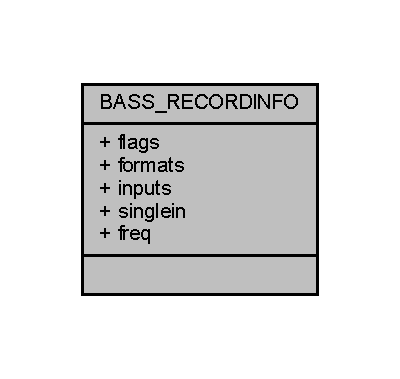
\includegraphics[width=192pt]{struct_b_a_s_s___r_e_c_o_r_d_i_n_f_o__coll__graph}
\end{center}
\end{figure}
\subsection*{Public Attributes}
\begin{DoxyCompactItemize}
\item 
\hypertarget{struct_b_a_s_s___r_e_c_o_r_d_i_n_f_o_a97ae96c797ff1c981b459506629bad9c_a97ae96c797ff1c981b459506629bad9c}{D\-W\-O\-R\-D {\bfseries flags}}\label{struct_b_a_s_s___r_e_c_o_r_d_i_n_f_o_a97ae96c797ff1c981b459506629bad9c_a97ae96c797ff1c981b459506629bad9c}

\item 
\hypertarget{struct_b_a_s_s___r_e_c_o_r_d_i_n_f_o_aedfae3cd5f0d09c239eda38ed3ef9c2b_aedfae3cd5f0d09c239eda38ed3ef9c2b}{D\-W\-O\-R\-D {\bfseries formats}}\label{struct_b_a_s_s___r_e_c_o_r_d_i_n_f_o_aedfae3cd5f0d09c239eda38ed3ef9c2b_aedfae3cd5f0d09c239eda38ed3ef9c2b}

\item 
\hypertarget{struct_b_a_s_s___r_e_c_o_r_d_i_n_f_o_a7b049b2bd7f57b9f8fba6f01c0106589_a7b049b2bd7f57b9f8fba6f01c0106589}{D\-W\-O\-R\-D {\bfseries inputs}}\label{struct_b_a_s_s___r_e_c_o_r_d_i_n_f_o_a7b049b2bd7f57b9f8fba6f01c0106589_a7b049b2bd7f57b9f8fba6f01c0106589}

\item 
\hypertarget{struct_b_a_s_s___r_e_c_o_r_d_i_n_f_o_a5a18b145e6f2bf4670cc815cea5744ec_a5a18b145e6f2bf4670cc815cea5744ec}{B\-O\-O\-L {\bfseries singlein}}\label{struct_b_a_s_s___r_e_c_o_r_d_i_n_f_o_a5a18b145e6f2bf4670cc815cea5744ec_a5a18b145e6f2bf4670cc815cea5744ec}

\item 
\hypertarget{struct_b_a_s_s___r_e_c_o_r_d_i_n_f_o_af643ddd16623da7b0370ab191d8bb204_af643ddd16623da7b0370ab191d8bb204}{D\-W\-O\-R\-D {\bfseries freq}}\label{struct_b_a_s_s___r_e_c_o_r_d_i_n_f_o_af643ddd16623da7b0370ab191d8bb204_af643ddd16623da7b0370ab191d8bb204}

\end{DoxyCompactItemize}


\subsection{Detailed Description}


Definition at line 194 of file bass.\-h.



The documentation for this struct was generated from the following files\-:\begin{DoxyCompactItemize}
\item 
D\-A\-W\-Components/bass.\-h\item 
M\-S\-Master\-Cmp/bass.\-h\end{DoxyCompactItemize}

\hypertarget{struct_b_a_s_s___s_a_m_p_l_e}{\section{B\-A\-S\-S\-\_\-\-S\-A\-M\-P\-L\-E Struct Reference}
\label{struct_b_a_s_s___s_a_m_p_l_e}\index{B\-A\-S\-S\-\_\-\-S\-A\-M\-P\-L\-E@{B\-A\-S\-S\-\_\-\-S\-A\-M\-P\-L\-E}}
}


Collaboration diagram for B\-A\-S\-S\-\_\-\-S\-A\-M\-P\-L\-E\-:\nopagebreak
\begin{figure}[H]
\begin{center}
\leavevmode
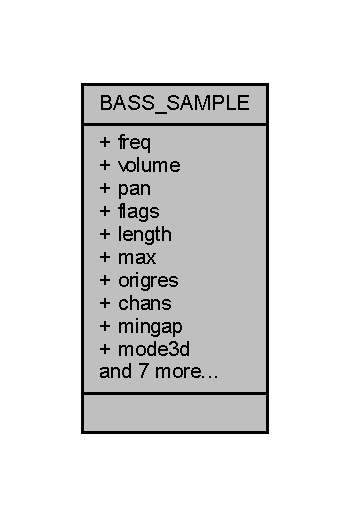
\includegraphics[width=168pt]{struct_b_a_s_s___s_a_m_p_l_e__coll__graph}
\end{center}
\end{figure}
\subsection*{Public Attributes}
\begin{DoxyCompactItemize}
\item 
\hypertarget{struct_b_a_s_s___s_a_m_p_l_e_acabd72a2635853202082a5ad0c9529e7_acabd72a2635853202082a5ad0c9529e7}{D\-W\-O\-R\-D {\bfseries freq}}\label{struct_b_a_s_s___s_a_m_p_l_e_acabd72a2635853202082a5ad0c9529e7_acabd72a2635853202082a5ad0c9529e7}

\item 
\hypertarget{struct_b_a_s_s___s_a_m_p_l_e_a44fc378a594c2eabb25fb54b0809d632_a44fc378a594c2eabb25fb54b0809d632}{float {\bfseries volume}}\label{struct_b_a_s_s___s_a_m_p_l_e_a44fc378a594c2eabb25fb54b0809d632_a44fc378a594c2eabb25fb54b0809d632}

\item 
\hypertarget{struct_b_a_s_s___s_a_m_p_l_e_aae9f6113048ac8c46c1b4b8de3d3e032_aae9f6113048ac8c46c1b4b8de3d3e032}{float {\bfseries pan}}\label{struct_b_a_s_s___s_a_m_p_l_e_aae9f6113048ac8c46c1b4b8de3d3e032_aae9f6113048ac8c46c1b4b8de3d3e032}

\item 
\hypertarget{struct_b_a_s_s___s_a_m_p_l_e_ae2863c9c7e8f3e40805cfb81759e9e51_ae2863c9c7e8f3e40805cfb81759e9e51}{D\-W\-O\-R\-D {\bfseries flags}}\label{struct_b_a_s_s___s_a_m_p_l_e_ae2863c9c7e8f3e40805cfb81759e9e51_ae2863c9c7e8f3e40805cfb81759e9e51}

\item 
\hypertarget{struct_b_a_s_s___s_a_m_p_l_e_afee703fb2be34e5ea6cd2d9a9e8ddff0_afee703fb2be34e5ea6cd2d9a9e8ddff0}{D\-W\-O\-R\-D {\bfseries length}}\label{struct_b_a_s_s___s_a_m_p_l_e_afee703fb2be34e5ea6cd2d9a9e8ddff0_afee703fb2be34e5ea6cd2d9a9e8ddff0}

\item 
\hypertarget{struct_b_a_s_s___s_a_m_p_l_e_a42ecc61ca6008579bc2fcb4fb1bc19fe_a42ecc61ca6008579bc2fcb4fb1bc19fe}{D\-W\-O\-R\-D {\bfseries max}}\label{struct_b_a_s_s___s_a_m_p_l_e_a42ecc61ca6008579bc2fcb4fb1bc19fe_a42ecc61ca6008579bc2fcb4fb1bc19fe}

\item 
\hypertarget{struct_b_a_s_s___s_a_m_p_l_e_a9f0c4c3caeab28316ead100cc6d36844_a9f0c4c3caeab28316ead100cc6d36844}{D\-W\-O\-R\-D {\bfseries origres}}\label{struct_b_a_s_s___s_a_m_p_l_e_a9f0c4c3caeab28316ead100cc6d36844_a9f0c4c3caeab28316ead100cc6d36844}

\item 
\hypertarget{struct_b_a_s_s___s_a_m_p_l_e_a0f7dc81cf0753dbe14848d61544e7f51_a0f7dc81cf0753dbe14848d61544e7f51}{D\-W\-O\-R\-D {\bfseries chans}}\label{struct_b_a_s_s___s_a_m_p_l_e_a0f7dc81cf0753dbe14848d61544e7f51_a0f7dc81cf0753dbe14848d61544e7f51}

\item 
\hypertarget{struct_b_a_s_s___s_a_m_p_l_e_a17646b031533f3ecb07ee5318b484f44_a17646b031533f3ecb07ee5318b484f44}{D\-W\-O\-R\-D {\bfseries mingap}}\label{struct_b_a_s_s___s_a_m_p_l_e_a17646b031533f3ecb07ee5318b484f44_a17646b031533f3ecb07ee5318b484f44}

\item 
\hypertarget{struct_b_a_s_s___s_a_m_p_l_e_a20fcedf825bd2d62cff1a39dd4a79d4f_a20fcedf825bd2d62cff1a39dd4a79d4f}{D\-W\-O\-R\-D {\bfseries mode3d}}\label{struct_b_a_s_s___s_a_m_p_l_e_a20fcedf825bd2d62cff1a39dd4a79d4f_a20fcedf825bd2d62cff1a39dd4a79d4f}

\item 
\hypertarget{struct_b_a_s_s___s_a_m_p_l_e_aae9039af2e1e14189bc6df67c89077de_aae9039af2e1e14189bc6df67c89077de}{float {\bfseries mindist}}\label{struct_b_a_s_s___s_a_m_p_l_e_aae9039af2e1e14189bc6df67c89077de_aae9039af2e1e14189bc6df67c89077de}

\item 
\hypertarget{struct_b_a_s_s___s_a_m_p_l_e_a3e3c1c0fc99110afd6b7cebbcab1ad35_a3e3c1c0fc99110afd6b7cebbcab1ad35}{float {\bfseries maxdist}}\label{struct_b_a_s_s___s_a_m_p_l_e_a3e3c1c0fc99110afd6b7cebbcab1ad35_a3e3c1c0fc99110afd6b7cebbcab1ad35}

\item 
\hypertarget{struct_b_a_s_s___s_a_m_p_l_e_a680ef402d0a1a1f934f35aa3eb74c746_a680ef402d0a1a1f934f35aa3eb74c746}{D\-W\-O\-R\-D {\bfseries iangle}}\label{struct_b_a_s_s___s_a_m_p_l_e_a680ef402d0a1a1f934f35aa3eb74c746_a680ef402d0a1a1f934f35aa3eb74c746}

\item 
\hypertarget{struct_b_a_s_s___s_a_m_p_l_e_a6fac12da5e3308d9122f0f8c9e7eb181_a6fac12da5e3308d9122f0f8c9e7eb181}{D\-W\-O\-R\-D {\bfseries oangle}}\label{struct_b_a_s_s___s_a_m_p_l_e_a6fac12da5e3308d9122f0f8c9e7eb181_a6fac12da5e3308d9122f0f8c9e7eb181}

\item 
\hypertarget{struct_b_a_s_s___s_a_m_p_l_e_a8c280d4cfbc49970503b931c9e8fa4dc_a8c280d4cfbc49970503b931c9e8fa4dc}{float {\bfseries outvol}}\label{struct_b_a_s_s___s_a_m_p_l_e_a8c280d4cfbc49970503b931c9e8fa4dc_a8c280d4cfbc49970503b931c9e8fa4dc}

\item 
\hypertarget{struct_b_a_s_s___s_a_m_p_l_e_af6bf250cbb800dfff363da346074e301_af6bf250cbb800dfff363da346074e301}{D\-W\-O\-R\-D {\bfseries vam}}\label{struct_b_a_s_s___s_a_m_p_l_e_af6bf250cbb800dfff363da346074e301_af6bf250cbb800dfff363da346074e301}

\item 
\hypertarget{struct_b_a_s_s___s_a_m_p_l_e_a99f47aeb64df3819f1c419a94a911a24_a99f47aeb64df3819f1c419a94a911a24}{D\-W\-O\-R\-D {\bfseries priority}}\label{struct_b_a_s_s___s_a_m_p_l_e_a99f47aeb64df3819f1c419a94a911a24_a99f47aeb64df3819f1c419a94a911a24}

\end{DoxyCompactItemize}


\subsection{Detailed Description}


Definition at line 223 of file bass.\-h.



The documentation for this struct was generated from the following files\-:\begin{DoxyCompactItemize}
\item 
D\-A\-W\-Components/bass.\-h\item 
M\-S\-Master\-Cmp/bass.\-h\end{DoxyCompactItemize}

\hypertarget{class_d_a_w_inputs_1_1_d_a_w_error}{\section{D\-A\-W\-Inputs\-:\-:D\-A\-W\-Error Class Reference}
\label{class_d_a_w_inputs_1_1_d_a_w_error}\index{D\-A\-W\-Inputs\-::\-D\-A\-W\-Error@{D\-A\-W\-Inputs\-::\-D\-A\-W\-Error}}
}


The \hyperlink{class_d_a_w_inputs_1_1_d_a_w_error}{D\-A\-W\-Error} class.  




{\ttfamily \#include $<$dawerror.\-h$>$}



Inheritance diagram for D\-A\-W\-Inputs\-:\-:D\-A\-W\-Error\-:
\nopagebreak
\begin{figure}[H]
\begin{center}
\leavevmode
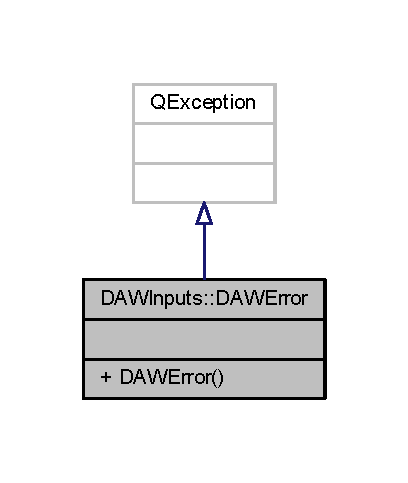
\includegraphics[width=196pt]{class_d_a_w_inputs_1_1_d_a_w_error__inherit__graph}
\end{center}
\end{figure}


Collaboration diagram for D\-A\-W\-Inputs\-:\-:D\-A\-W\-Error\-:
\nopagebreak
\begin{figure}[H]
\begin{center}
\leavevmode
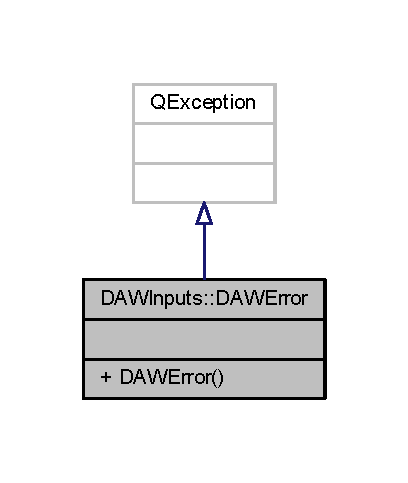
\includegraphics[width=196pt]{class_d_a_w_inputs_1_1_d_a_w_error__coll__graph}
\end{center}
\end{figure}


\subsection{Detailed Description}
The \hyperlink{class_d_a_w_inputs_1_1_d_a_w_error}{D\-A\-W\-Error} class. 

Definition at line 11 of file dawerror.\-h.



The documentation for this class was generated from the following files\-:\begin{DoxyCompactItemize}
\item 
D\-A\-W\-Components/dawerror.\-h\item 
D\-A\-W\-Components/dawerror.\-cpp\end{DoxyCompactItemize}

\hypertarget{class_d_a_w_inputs_1_1_file_input}{\section{D\-A\-W\-Inputs\-:\-:File\-Input Class Reference}
\label{class_d_a_w_inputs_1_1_file_input}\index{D\-A\-W\-Inputs\-::\-File\-Input@{D\-A\-W\-Inputs\-::\-File\-Input}}
}


The \hyperlink{class_d_a_w_inputs_1_1_file_input}{File\-Input} class.  




{\ttfamily \#include $<$fileinput.\-h$>$}



Inheritance diagram for D\-A\-W\-Inputs\-:\-:File\-Input\-:
\nopagebreak
\begin{figure}[H]
\begin{center}
\leavevmode
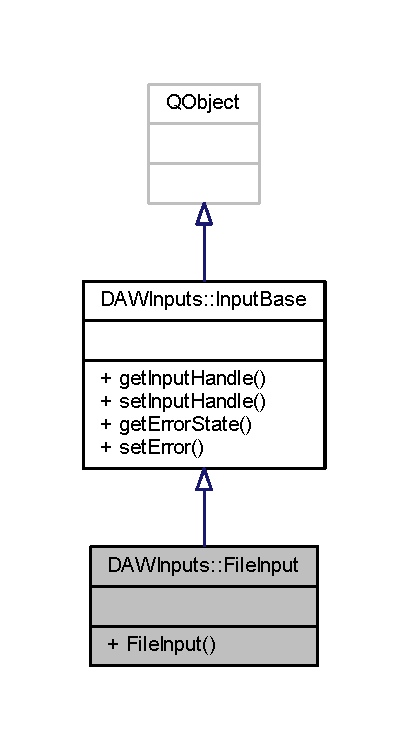
\includegraphics[width=196pt]{class_d_a_w_inputs_1_1_file_input__inherit__graph}
\end{center}
\end{figure}


Collaboration diagram for D\-A\-W\-Inputs\-:\-:File\-Input\-:
\nopagebreak
\begin{figure}[H]
\begin{center}
\leavevmode
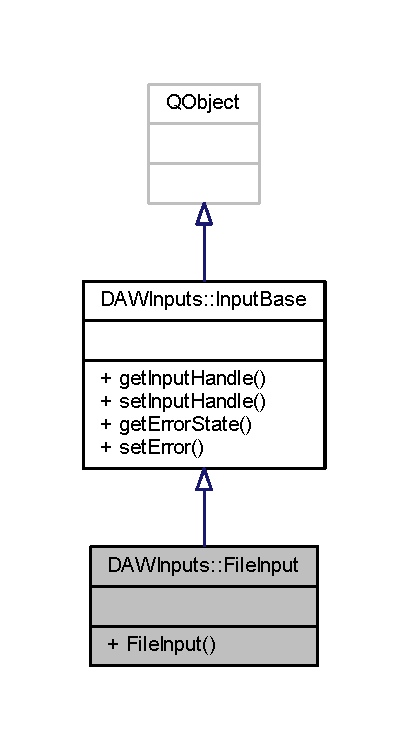
\includegraphics[width=196pt]{class_d_a_w_inputs_1_1_file_input__coll__graph}
\end{center}
\end{figure}
\subsection*{Public Member Functions}
\begin{DoxyCompactItemize}
\item 
\hyperlink{class_d_a_w_inputs_1_1_file_input_a5a18fa8381fb317541c12ca49d0d1a29_a5a18fa8381fb317541c12ca49d0d1a29}{File\-Input} (Q\-String $\ast$file, B\-O\-O\-L mem=false, Q\-W\-O\-R\-D offset=0, Q\-W\-O\-R\-D length=0, D\-W\-O\-R\-D flags=B\-A\-S\-S\-\_\-\-S\-T\-R\-E\-A\-M\-\_\-\-D\-E\-C\-O\-D\-E$|$B\-A\-S\-S\-\_\-\-S\-A\-M\-P\-L\-E\-\_\-\-F\-L\-O\-A\-T$|$B\-A\-S\-S\-\_\-\-A\-S\-Y\-N\-C\-F\-I\-L\-E)
\begin{DoxyCompactList}\small\item\em \hyperlink{class_d_a_w_inputs_1_1_file_input}{File\-Input}. \end{DoxyCompactList}\end{DoxyCompactItemize}
\subsection*{Additional Inherited Members}


\subsection{Detailed Description}
The \hyperlink{class_d_a_w_inputs_1_1_file_input}{File\-Input} class. 

Definition at line 12 of file fileinput.\-h.



\subsection{Constructor \& Destructor Documentation}
\hypertarget{class_d_a_w_inputs_1_1_file_input_a5a18fa8381fb317541c12ca49d0d1a29_a5a18fa8381fb317541c12ca49d0d1a29}{\index{D\-A\-W\-Inputs\-::\-File\-Input@{D\-A\-W\-Inputs\-::\-File\-Input}!File\-Input@{File\-Input}}
\index{File\-Input@{File\-Input}!DAWInputs::FileInput@{D\-A\-W\-Inputs\-::\-File\-Input}}
\subsubsection[{File\-Input}]{\setlength{\rightskip}{0pt plus 5cm}D\-A\-W\-Inputs\-::\-File\-Input\-::\-File\-Input (
\begin{DoxyParamCaption}
\item[{Q\-String $\ast$}]{file, }
\item[{B\-O\-O\-L}]{mem = {\ttfamily false}, }
\item[{Q\-W\-O\-R\-D}]{offset = {\ttfamily 0}, }
\item[{Q\-W\-O\-R\-D}]{length = {\ttfamily 0}, }
\item[{D\-W\-O\-R\-D}]{flags = {\ttfamily BASS\-\_\-STREAM\-\_\-DECODE~$|$~BASS\-\_\-SAMPLE\-\_\-FLOAT~$|$~BASS\-\_\-ASYNCFILE}}
\end{DoxyParamCaption}
)}}\label{class_d_a_w_inputs_1_1_file_input_a5a18fa8381fb317541c12ca49d0d1a29_a5a18fa8381fb317541c12ca49d0d1a29}


\hyperlink{class_d_a_w_inputs_1_1_file_input}{File\-Input}. 


\begin{DoxyParams}{Parameters}
{\em file} & \\
\hline
{\em mem} & \\
\hline
{\em offset} & \\
\hline
{\em length} & \\
\hline
{\em flags} & \\
\hline
\end{DoxyParams}


Definition at line 3 of file fileinput.\-cpp.


\begin{DoxyCode}
4 \{
5     this->setInputHandle(BASS\_StreamCreateFile(mem, file, offset, length, flags));
6 \}
\end{DoxyCode}


The documentation for this class was generated from the following files\-:\begin{DoxyCompactItemize}
\item 
D\-A\-W\-Components/fileinput.\-h\item 
D\-A\-W\-Components/fileinput.\-cpp\end{DoxyCompactItemize}

\hypertarget{class_d_a_w_inputs_1_1_input_base}{\section{D\-A\-W\-Inputs\-:\-:Input\-Base Class Reference}
\label{class_d_a_w_inputs_1_1_input_base}\index{D\-A\-W\-Inputs\-::\-Input\-Base@{D\-A\-W\-Inputs\-::\-Input\-Base}}
}


Inheritance diagram for D\-A\-W\-Inputs\-:\-:Input\-Base\-:
\nopagebreak
\begin{figure}[H]
\begin{center}
\leavevmode
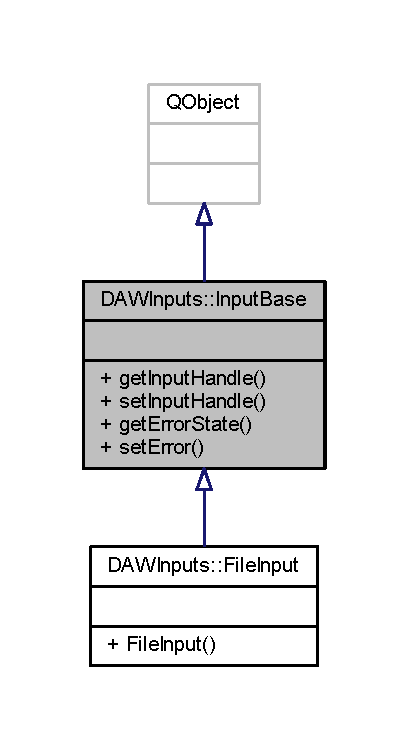
\includegraphics[width=196pt]{class_d_a_w_inputs_1_1_input_base__inherit__graph}
\end{center}
\end{figure}


Collaboration diagram for D\-A\-W\-Inputs\-:\-:Input\-Base\-:
\nopagebreak
\begin{figure}[H]
\begin{center}
\leavevmode
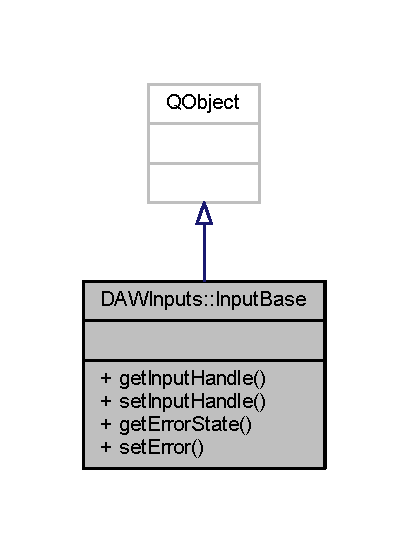
\includegraphics[width=196pt]{class_d_a_w_inputs_1_1_input_base__coll__graph}
\end{center}
\end{figure}
\subsection*{Public Slots}
\begin{DoxyCompactItemize}
\item 
\hypertarget{class_d_a_w_inputs_1_1_input_base_ac7c056c9082dc4de0140a939bca469da_ac7c056c9082dc4de0140a939bca469da}{void {\bfseries set\-Error} (bool error)}\label{class_d_a_w_inputs_1_1_input_base_ac7c056c9082dc4de0140a939bca469da_ac7c056c9082dc4de0140a939bca469da}

\end{DoxyCompactItemize}
\subsection*{Public Member Functions}
\begin{DoxyCompactItemize}
\item 
\hypertarget{class_d_a_w_inputs_1_1_input_base_a73224efbabf4aad4b0895bcf51ba70d8_a73224efbabf4aad4b0895bcf51ba70d8}{const D\-W\-O\-R\-D {\bfseries get\-Input\-Handle} ()}\label{class_d_a_w_inputs_1_1_input_base_a73224efbabf4aad4b0895bcf51ba70d8_a73224efbabf4aad4b0895bcf51ba70d8}

\item 
\hypertarget{class_d_a_w_inputs_1_1_input_base_a95951cffd8b18decc69565cca4fa7551_a95951cffd8b18decc69565cca4fa7551}{void {\bfseries set\-Input\-Handle} (D\-W\-O\-R\-D handle)}\label{class_d_a_w_inputs_1_1_input_base_a95951cffd8b18decc69565cca4fa7551_a95951cffd8b18decc69565cca4fa7551}

\item 
\hypertarget{class_d_a_w_inputs_1_1_input_base_aad8f817d8e43f71d92d7cbd8eb360eb1_aad8f817d8e43f71d92d7cbd8eb360eb1}{bool {\bfseries get\-Error\-State} ()}\label{class_d_a_w_inputs_1_1_input_base_aad8f817d8e43f71d92d7cbd8eb360eb1_aad8f817d8e43f71d92d7cbd8eb360eb1}

\end{DoxyCompactItemize}


\subsection{Detailed Description}


Definition at line 9 of file dawinput.\-h.



The documentation for this class was generated from the following files\-:\begin{DoxyCompactItemize}
\item 
D\-A\-W\-Components/dawinput.\-h\item 
D\-A\-W\-Components/dawinput.\-cpp\end{DoxyCompactItemize}

\hypertarget{class_m_s_master_error}{\section{M\-S\-Master\-Error Class Reference}
\label{class_m_s_master_error}\index{M\-S\-Master\-Error@{M\-S\-Master\-Error}}
}


The \hyperlink{class_m_s_master_error}{M\-S\-Master\-Error} class Thrown by the M\-S\-Master\-Components. Contains Information about the errors occured in those components.  




{\ttfamily \#include $<$msmastererror.\-h$>$}



Inheritance diagram for M\-S\-Master\-Error\-:\nopagebreak
\begin{figure}[H]
\begin{center}
\leavevmode
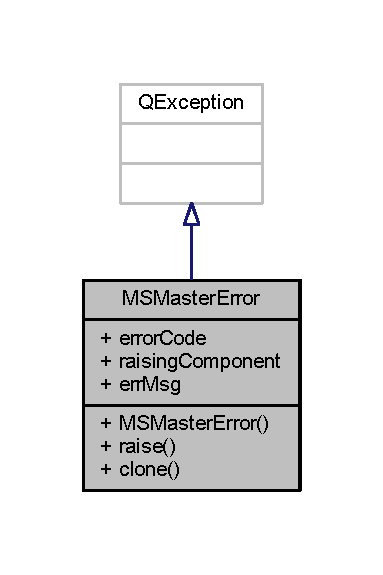
\includegraphics[width=184pt]{class_m_s_master_error__inherit__graph}
\end{center}
\end{figure}


Collaboration diagram for M\-S\-Master\-Error\-:\nopagebreak
\begin{figure}[H]
\begin{center}
\leavevmode
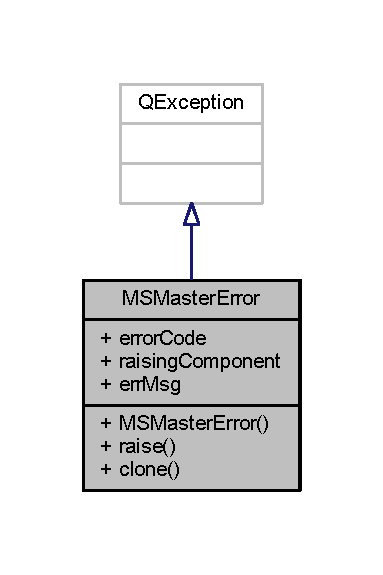
\includegraphics[width=184pt]{class_m_s_master_error__coll__graph}
\end{center}
\end{figure}
\subsection*{Public Types}
\begin{DoxyCompactItemize}
\item 
enum \hyperlink{class_m_s_master_error_aa1deb878016117b72d744363b49a16e4_aa1deb878016117b72d744363b49a16e4}{M\-S\-M\-A\-S\-T\-E\-R\-\_\-\-E\-R\-R\-O\-R\-\_\-\-C\-O\-D\-E} \{ {\bfseries Unknown\-\_\-\-Error}, 
{\bfseries Channel\-Remove\-\_\-\-Error}, 
{\bfseries Add\-Channel\-\_\-\-Error}, 
{\bfseries Set\-Matrix\-\_\-\-Error}
 \}
\begin{DoxyCompactList}\small\item\em The M\-S\-M\-A\-S\-T\-E\-R\-\_\-\-E\-R\-R\-O\-R\-\_\-\-C\-O\-D\-E enum. \end{DoxyCompactList}\end{DoxyCompactItemize}
\subsection*{Public Member Functions}
\begin{DoxyCompactItemize}
\item 
\hypertarget{class_m_s_master_error_ae99de5e65ace36645a5f4979c4e91e8e_ae99de5e65ace36645a5f4979c4e91e8e}{{\bfseries M\-S\-Master\-Error} (\hyperlink{class_m_s_master_error_aa1deb878016117b72d744363b49a16e4_aa1deb878016117b72d744363b49a16e4}{M\-S\-Master\-Error\-::\-M\-S\-M\-A\-S\-T\-E\-R\-\_\-\-E\-R\-R\-O\-R\-\_\-\-C\-O\-D\-E} ec, Q\-String $\ast$cmp, Q\-String $\ast$error\-Msg)}\label{class_m_s_master_error_ae99de5e65ace36645a5f4979c4e91e8e_ae99de5e65ace36645a5f4979c4e91e8e}

\item 
\hypertarget{class_m_s_master_error_aa3f4ef6e72be82c5600cc0a2ced741be_aa3f4ef6e72be82c5600cc0a2ced741be}{void {\bfseries raise} () const }\label{class_m_s_master_error_aa3f4ef6e72be82c5600cc0a2ced741be_aa3f4ef6e72be82c5600cc0a2ced741be}

\item 
\hypertarget{class_m_s_master_error_aa217c96d2f3cc8e2d1e1fc98f7f63061_aa217c96d2f3cc8e2d1e1fc98f7f63061}{\hyperlink{class_m_s_master_error}{M\-S\-Master\-Error} $\ast$ {\bfseries clone} () const }\label{class_m_s_master_error_aa217c96d2f3cc8e2d1e1fc98f7f63061_aa217c96d2f3cc8e2d1e1fc98f7f63061}

\end{DoxyCompactItemize}
\subsection*{Public Attributes}
\begin{DoxyCompactItemize}
\item 
\hypertarget{class_m_s_master_error_ad600de0b538d634c7ce5ea94eb2ce49a_ad600de0b538d634c7ce5ea94eb2ce49a}{\hyperlink{class_m_s_master_error_aa1deb878016117b72d744363b49a16e4_aa1deb878016117b72d744363b49a16e4}{M\-S\-M\-A\-S\-T\-E\-R\-\_\-\-E\-R\-R\-O\-R\-\_\-\-C\-O\-D\-E} {\bfseries error\-Code}}\label{class_m_s_master_error_ad600de0b538d634c7ce5ea94eb2ce49a_ad600de0b538d634c7ce5ea94eb2ce49a}

\item 
\hypertarget{class_m_s_master_error_a14899875fb763876453cfc8f781c1a03_a14899875fb763876453cfc8f781c1a03}{Q\-String $\ast$ {\bfseries raising\-Component}}\label{class_m_s_master_error_a14899875fb763876453cfc8f781c1a03_a14899875fb763876453cfc8f781c1a03}

\item 
\hypertarget{class_m_s_master_error_a05456d32a4ac9b5d5eddf1b90f1a67bd_a05456d32a4ac9b5d5eddf1b90f1a67bd}{Q\-String $\ast$ {\bfseries err\-Msg}}\label{class_m_s_master_error_a05456d32a4ac9b5d5eddf1b90f1a67bd_a05456d32a4ac9b5d5eddf1b90f1a67bd}

\end{DoxyCompactItemize}


\subsection{Detailed Description}
The \hyperlink{class_m_s_master_error}{M\-S\-Master\-Error} class Thrown by the M\-S\-Master\-Components. Contains Information about the errors occured in those components. 

Definition at line 11 of file msmastererror.\-h.



The documentation for this class was generated from the following files\-:\begin{DoxyCompactItemize}
\item 
M\-S\-Master\-Cmp/msmastererror.\-h\item 
M\-S\-Master\-Cmp/M\-S\-Master\-Error.\-cpp\end{DoxyCompactItemize}

\hypertarget{class_m_s_master_splitter}{\section{M\-S\-Master\-Splitter Class Reference}
\label{class_m_s_master_splitter}\index{M\-S\-Master\-Splitter@{M\-S\-Master\-Splitter}}
}


The \hyperlink{class_m_s_master_splitter}{M\-S\-Master\-Splitter} class uses a mixer to create a stereo stream that at the left channel mixes the sideband and at the right the midband(the mono signal). The resulting stream is send to a splitterstream that creates two outputstreams(0=S, 1=M).  




{\ttfamily \#include $<$msmastercmp.\-h$>$}



Collaboration diagram for M\-S\-Master\-Splitter\-:\nopagebreak
\begin{figure}[H]
\begin{center}
\leavevmode
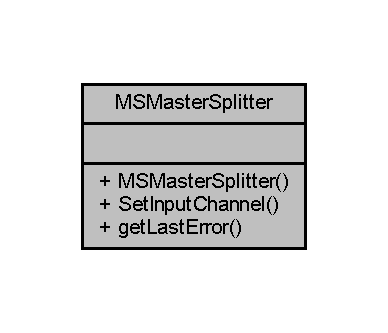
\includegraphics[width=186pt]{class_m_s_master_splitter__coll__graph}
\end{center}
\end{figure}
\subsection*{Public Member Functions}
\begin{DoxyCompactItemize}
\item 
\hyperlink{class_m_s_master_splitter_abb9f371e43978f5d0c8746d35e8debb4_abb9f371e43978f5d0c8746d35e8debb4}{M\-S\-Master\-Splitter} (D\-W\-O\-R\-D freq, D\-W\-O\-R\-D mixer\-Flags=256$|$0x200000, D\-W\-O\-R\-D splitter\-Flags=0x200000)
\begin{DoxyCompactList}\small\item\em \hyperlink{class_m_s_master_splitter}{M\-S\-Master\-Splitter}. \end{DoxyCompactList}\item 
bool \hyperlink{class_m_s_master_splitter_ae3fbab075c1c6872ba503f18c92ac792_ae3fbab075c1c6872ba503f18c92ac792}{Set\-Input\-Channel} (D\-W\-O\-R\-D channel, D\-W\-O\-R\-D flags=0x10000)
\begin{DoxyCompactList}\small\item\em Set\-Input\-Channel Sets the inputchannel for the mixer. If a channel is already applied this channel will be replaced by the new one. \end{DoxyCompactList}\item 
\hypertarget{class_m_s_master_splitter_ab903ca4a666f5702d79eab169d65cc27_ab903ca4a666f5702d79eab169d65cc27}{const \hyperlink{class_m_s_master_error}{M\-S\-Master\-Error} $\ast$ {\bfseries get\-Last\-Error} ()}\label{class_m_s_master_splitter_ab903ca4a666f5702d79eab169d65cc27_ab903ca4a666f5702d79eab169d65cc27}

\end{DoxyCompactItemize}


\subsection{Detailed Description}
The \hyperlink{class_m_s_master_splitter}{M\-S\-Master\-Splitter} class uses a mixer to create a stereo stream that at the left channel mixes the sideband and at the right the midband(the mono signal). The resulting stream is send to a splitterstream that creates two outputstreams(0=S, 1=M). 

Definition at line 13 of file msmastercmp.\-h.



\subsection{Constructor \& Destructor Documentation}
\hypertarget{class_m_s_master_splitter_abb9f371e43978f5d0c8746d35e8debb4_abb9f371e43978f5d0c8746d35e8debb4}{\index{M\-S\-Master\-Splitter@{M\-S\-Master\-Splitter}!M\-S\-Master\-Splitter@{M\-S\-Master\-Splitter}}
\index{M\-S\-Master\-Splitter@{M\-S\-Master\-Splitter}!MSMasterSplitter@{M\-S\-Master\-Splitter}}
\subsubsection[{M\-S\-Master\-Splitter}]{\setlength{\rightskip}{0pt plus 5cm}M\-S\-Master\-Splitter\-::\-M\-S\-Master\-Splitter (
\begin{DoxyParamCaption}
\item[{D\-W\-O\-R\-D}]{freq, }
\item[{D\-W\-O\-R\-D}]{mixer\-Flags = {\ttfamily 256~$|$~0x200000}, }
\item[{D\-W\-O\-R\-D}]{splitter\-Flags = {\ttfamily 0x200000}}
\end{DoxyParamCaption}
)}}\label{class_m_s_master_splitter_abb9f371e43978f5d0c8746d35e8debb4_abb9f371e43978f5d0c8746d35e8debb4}


\hyperlink{class_m_s_master_splitter}{M\-S\-Master\-Splitter}. 


\begin{DoxyParams}{Parameters}
{\em freq} & the sample rate of the mixer \\
\hline
{\em mixer\-Flags} & flags used by the mixer. For more information see the bassmix documentation. \\
\hline
{\em splitter\-Flags} & flags used by the splitter. More info see basmix documentation. \\
\hline
\end{DoxyParams}


Definition at line 4 of file msmastercmp.\-cpp.


\begin{DoxyCode}
5     :\_curInpChannel(0)
6 \{
7     \_mixerHandle=BASS\_Mixer\_StreamCreate(freq,2,mixerFlags);
8     \textcolor{keywordtype}{int} chanMap[]=\{0,1,-1\};
9     \_msSplitter=BASS\_Split\_StreamCreate(\_mixerHandle,splitterFlags,chanMap);
10 
11 \}
\end{DoxyCode}


\subsection{Member Function Documentation}
\hypertarget{class_m_s_master_splitter_ae3fbab075c1c6872ba503f18c92ac792_ae3fbab075c1c6872ba503f18c92ac792}{\index{M\-S\-Master\-Splitter@{M\-S\-Master\-Splitter}!Set\-Input\-Channel@{Set\-Input\-Channel}}
\index{Set\-Input\-Channel@{Set\-Input\-Channel}!MSMasterSplitter@{M\-S\-Master\-Splitter}}
\subsubsection[{Set\-Input\-Channel}]{\setlength{\rightskip}{0pt plus 5cm}bool M\-S\-Master\-Splitter\-::\-Set\-Input\-Channel (
\begin{DoxyParamCaption}
\item[{D\-W\-O\-R\-D}]{channel, }
\item[{D\-W\-O\-R\-D}]{flags = {\ttfamily 0x10000}}
\end{DoxyParamCaption}
)}}\label{class_m_s_master_splitter_ae3fbab075c1c6872ba503f18c92ac792_ae3fbab075c1c6872ba503f18c92ac792}


Set\-Input\-Channel Sets the inputchannel for the mixer. If a channel is already applied this channel will be replaced by the new one. 


\begin{DoxyParams}{Parameters}
{\em channel} & the channel to plugin to the mixer. \\
\hline
{\em flags} & for more info see bassmix documentation. \\
\hline
\end{DoxyParams}
\begin{DoxyReturn}{Returns}
true if succesful else false. 
\end{DoxyReturn}


Definition at line 13 of file msmastercmp.\-cpp.


\begin{DoxyCode}
13                                                                 \{
14     \textcolor{keywordflow}{if}(\_curInpChannel != 0)\{
15         \textcolor{keywordflow}{if}(BASS\_Mixer\_ChannelRemove(\_curInpChannel))\{
16             \_curInpChannel=0;
17         \}
18         \textcolor{keywordflow}{else}\{
19             \_lastError=\textcolor{keyword}{new} \hyperlink{class_m_s_master_error}{MSMasterError}(MSMasterError::ChannelRemove\_Error,\textcolor{keyword}{new} QString(\textcolor{stringliteral}{"
      MSMasterSplitter"}),\textcolor{keyword}{new} QString(\textcolor{stringliteral}{"Unable to remove current channel!"}));
20             \_lastError->raise();
21             \textcolor{keywordflow}{return} \textcolor{keyword}{false};
22         \}
23     \}
24     \textcolor{keywordflow}{if}(!BASS\_Mixer\_StreamAddChannel(\_mixerHandle,channel,flags))\{
25         \_lastError=\textcolor{keyword}{new} \hyperlink{class_m_s_master_error}{MSMasterError}(MSMasterError::AddChannel\_Error, \textcolor{keyword}{new} QString(\textcolor{stringliteral}{"
      MSMasterSplitter"}), \textcolor{keyword}{new} QString(\textcolor{stringliteral}{"Setting input channel failed!"}));
26         \_lastError->raise();
27         \textcolor{keywordflow}{return} \textcolor{keyword}{false};
28     \}
29     \textcolor{keywordtype}{float} matrix[2][2]=\{
30         \{0,-1\},
31         \{0,1\}
32     \};
33     \textcolor{keywordflow}{if}(!BASS\_Mixer\_ChannelSetMatrix(channel, *matrix))\{
34         \_lastError=\textcolor{keyword}{new} \hyperlink{class_m_s_master_error}{MSMasterError}(MSMasterError::SetMatrix\_Error, \textcolor{keyword}{new} QString(\textcolor{stringliteral}{"
      MSMasterSplitter"}), \textcolor{keyword}{new} QString(\textcolor{stringliteral}{"Unable to set matrix on Channel!"}));
35         \_lastError->raise();
36         \textcolor{keywordflow}{return} \textcolor{keyword}{false};
37     \}
38     \textcolor{keywordflow}{return} \textcolor{keyword}{true};
39 \}
\end{DoxyCode}


The documentation for this class was generated from the following files\-:\begin{DoxyCompactItemize}
\item 
M\-S\-Master\-Cmp/msmastercmp.\-h\item 
M\-S\-Master\-Cmp/msmastercmp.\-cpp\end{DoxyCompactItemize}

\hypertarget{struct_t_a_g___a_p_e___b_i_n_a_r_y}{\section{T\-A\-G\-\_\-\-A\-P\-E\-\_\-\-B\-I\-N\-A\-R\-Y Struct Reference}
\label{struct_t_a_g___a_p_e___b_i_n_a_r_y}\index{T\-A\-G\-\_\-\-A\-P\-E\-\_\-\-B\-I\-N\-A\-R\-Y@{T\-A\-G\-\_\-\-A\-P\-E\-\_\-\-B\-I\-N\-A\-R\-Y}}
}


Collaboration diagram for T\-A\-G\-\_\-\-A\-P\-E\-\_\-\-B\-I\-N\-A\-R\-Y\-:\nopagebreak
\begin{figure}[H]
\begin{center}
\leavevmode
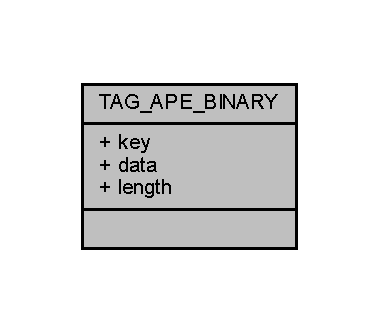
\includegraphics[width=182pt]{struct_t_a_g___a_p_e___b_i_n_a_r_y__coll__graph}
\end{center}
\end{figure}
\subsection*{Public Attributes}
\begin{DoxyCompactItemize}
\item 
\hypertarget{struct_t_a_g___a_p_e___b_i_n_a_r_y_a851f32ddd93b19c89274b475f85d884d_a851f32ddd93b19c89274b475f85d884d}{const char $\ast$ {\bfseries key}}\label{struct_t_a_g___a_p_e___b_i_n_a_r_y_a851f32ddd93b19c89274b475f85d884d_a851f32ddd93b19c89274b475f85d884d}

\item 
\hypertarget{struct_t_a_g___a_p_e___b_i_n_a_r_y_a98bd1044d1225d1d194e40242639f829_a98bd1044d1225d1d194e40242639f829}{const void $\ast$ {\bfseries data}}\label{struct_t_a_g___a_p_e___b_i_n_a_r_y_a98bd1044d1225d1d194e40242639f829_a98bd1044d1225d1d194e40242639f829}

\item 
\hypertarget{struct_t_a_g___a_p_e___b_i_n_a_r_y_a7e3623a188e60d152fb9cdcd7a8f9668_a7e3623a188e60d152fb9cdcd7a8f9668}{D\-W\-O\-R\-D {\bfseries length}}\label{struct_t_a_g___a_p_e___b_i_n_a_r_y_a7e3623a188e60d152fb9cdcd7a8f9668_a7e3623a188e60d152fb9cdcd7a8f9668}

\end{DoxyCompactItemize}


\subsection{Detailed Description}


Definition at line 620 of file bass.\-h.



The documentation for this struct was generated from the following files\-:\begin{DoxyCompactItemize}
\item 
D\-A\-W\-Components/bass.\-h\item 
M\-S\-Master\-Cmp/bass.\-h\end{DoxyCompactItemize}

\hypertarget{struct_t_a_g___b_e_x_t}{\section{T\-A\-G\-\_\-\-B\-E\-X\-T Struct Reference}
\label{struct_t_a_g___b_e_x_t}\index{T\-A\-G\-\_\-\-B\-E\-X\-T@{T\-A\-G\-\_\-\-B\-E\-X\-T}}
}


Collaboration diagram for T\-A\-G\-\_\-\-B\-E\-X\-T\-:\nopagebreak
\begin{figure}[H]
\begin{center}
\leavevmode
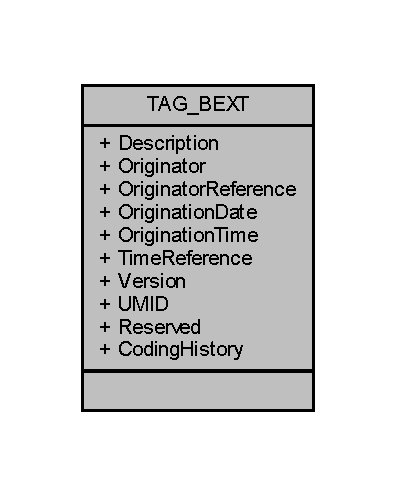
\includegraphics[width=190pt]{struct_t_a_g___b_e_x_t__coll__graph}
\end{center}
\end{figure}
\subsection*{Public Attributes}
\begin{DoxyCompactItemize}
\item 
\hypertarget{struct_t_a_g___b_e_x_t_a62583faae38b559bea3704363c139876_a62583faae38b559bea3704363c139876}{char {\bfseries Description} \mbox{[}256\mbox{]}}\label{struct_t_a_g___b_e_x_t_a62583faae38b559bea3704363c139876_a62583faae38b559bea3704363c139876}

\item 
\hypertarget{struct_t_a_g___b_e_x_t_a914e37d4230121eb898936e192199c61_a914e37d4230121eb898936e192199c61}{char {\bfseries Originator} \mbox{[}32\mbox{]}}\label{struct_t_a_g___b_e_x_t_a914e37d4230121eb898936e192199c61_a914e37d4230121eb898936e192199c61}

\item 
\hypertarget{struct_t_a_g___b_e_x_t_a6c057865f90093f08ff9f76a3c81c0b4_a6c057865f90093f08ff9f76a3c81c0b4}{char {\bfseries Originator\-Reference} \mbox{[}32\mbox{]}}\label{struct_t_a_g___b_e_x_t_a6c057865f90093f08ff9f76a3c81c0b4_a6c057865f90093f08ff9f76a3c81c0b4}

\item 
\hypertarget{struct_t_a_g___b_e_x_t_a3016f939d3c15c81b300329ff0df8842_a3016f939d3c15c81b300329ff0df8842}{char {\bfseries Origination\-Date} \mbox{[}10\mbox{]}}\label{struct_t_a_g___b_e_x_t_a3016f939d3c15c81b300329ff0df8842_a3016f939d3c15c81b300329ff0df8842}

\item 
\hypertarget{struct_t_a_g___b_e_x_t_a2d3294325a02b3a474f812c92f6f4b9c_a2d3294325a02b3a474f812c92f6f4b9c}{char {\bfseries Origination\-Time} \mbox{[}8\mbox{]}}\label{struct_t_a_g___b_e_x_t_a2d3294325a02b3a474f812c92f6f4b9c_a2d3294325a02b3a474f812c92f6f4b9c}

\item 
\hypertarget{struct_t_a_g___b_e_x_t_abae4961b0ac06cad4e7df0b0ad80c4df_abae4961b0ac06cad4e7df0b0ad80c4df}{Q\-W\-O\-R\-D {\bfseries Time\-Reference}}\label{struct_t_a_g___b_e_x_t_abae4961b0ac06cad4e7df0b0ad80c4df_abae4961b0ac06cad4e7df0b0ad80c4df}

\item 
\hypertarget{struct_t_a_g___b_e_x_t_a2f1751b9b0e537006ce9ee3c1dd001f9_a2f1751b9b0e537006ce9ee3c1dd001f9}{W\-O\-R\-D {\bfseries Version}}\label{struct_t_a_g___b_e_x_t_a2f1751b9b0e537006ce9ee3c1dd001f9_a2f1751b9b0e537006ce9ee3c1dd001f9}

\item 
\hypertarget{struct_t_a_g___b_e_x_t_a3aa7ac7da2b51c4747c9672ecc9f0b41_a3aa7ac7da2b51c4747c9672ecc9f0b41}{B\-Y\-T\-E {\bfseries U\-M\-I\-D} \mbox{[}64\mbox{]}}\label{struct_t_a_g___b_e_x_t_a3aa7ac7da2b51c4747c9672ecc9f0b41_a3aa7ac7da2b51c4747c9672ecc9f0b41}

\item 
\hypertarget{struct_t_a_g___b_e_x_t_aa752e8298cc5ecf8ce3bd2698d6307a0_aa752e8298cc5ecf8ce3bd2698d6307a0}{B\-Y\-T\-E {\bfseries Reserved} \mbox{[}190\mbox{]}}\label{struct_t_a_g___b_e_x_t_aa752e8298cc5ecf8ce3bd2698d6307a0_aa752e8298cc5ecf8ce3bd2698d6307a0}

\item 
\hypertarget{struct_t_a_g___b_e_x_t_a015b227447c52eb1ff4c3e6e9d0225de_a015b227447c52eb1ff4c3e6e9d0225de}{char {\bfseries Coding\-History} \mbox{[}$\,$\mbox{]}}\label{struct_t_a_g___b_e_x_t_a015b227447c52eb1ff4c3e6e9d0225de_a015b227447c52eb1ff4c3e6e9d0225de}

\end{DoxyCompactItemize}


\subsection{Detailed Description}


Definition at line 632 of file bass.\-h.



The documentation for this struct was generated from the following files\-:\begin{DoxyCompactItemize}
\item 
D\-A\-W\-Components/bass.\-h\item 
M\-S\-Master\-Cmp/bass.\-h\end{DoxyCompactItemize}

\hypertarget{struct_t_a_g___c_a___c_o_d_e_c}{\section{T\-A\-G\-\_\-\-C\-A\-\_\-\-C\-O\-D\-E\-C Struct Reference}
\label{struct_t_a_g___c_a___c_o_d_e_c}\index{T\-A\-G\-\_\-\-C\-A\-\_\-\-C\-O\-D\-E\-C@{T\-A\-G\-\_\-\-C\-A\-\_\-\-C\-O\-D\-E\-C}}
}


Collaboration diagram for T\-A\-G\-\_\-\-C\-A\-\_\-\-C\-O\-D\-E\-C\-:\nopagebreak
\begin{figure}[H]
\begin{center}
\leavevmode
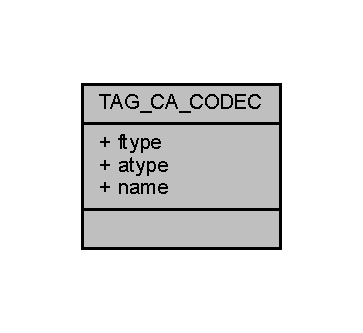
\includegraphics[width=174pt]{struct_t_a_g___c_a___c_o_d_e_c__coll__graph}
\end{center}
\end{figure}
\subsection*{Public Attributes}
\begin{DoxyCompactItemize}
\item 
\hypertarget{struct_t_a_g___c_a___c_o_d_e_c_af43a0d3c8d295bc3a37ae9245a47619b_af43a0d3c8d295bc3a37ae9245a47619b}{D\-W\-O\-R\-D {\bfseries ftype}}\label{struct_t_a_g___c_a___c_o_d_e_c_af43a0d3c8d295bc3a37ae9245a47619b_af43a0d3c8d295bc3a37ae9245a47619b}

\item 
\hypertarget{struct_t_a_g___c_a___c_o_d_e_c_a9f3c5b7726d72f1174290dfca6793bc1_a9f3c5b7726d72f1174290dfca6793bc1}{D\-W\-O\-R\-D {\bfseries atype}}\label{struct_t_a_g___c_a___c_o_d_e_c_a9f3c5b7726d72f1174290dfca6793bc1_a9f3c5b7726d72f1174290dfca6793bc1}

\item 
\hypertarget{struct_t_a_g___c_a___c_o_d_e_c_a75fc5f7cffd6b44cd32563d23b4bfa5e_a75fc5f7cffd6b44cd32563d23b4bfa5e}{const char $\ast$ {\bfseries name}}\label{struct_t_a_g___c_a___c_o_d_e_c_a75fc5f7cffd6b44cd32563d23b4bfa5e_a75fc5f7cffd6b44cd32563d23b4bfa5e}

\end{DoxyCompactItemize}


\subsection{Detailed Description}


Definition at line 693 of file bass.\-h.



The documentation for this struct was generated from the following files\-:\begin{DoxyCompactItemize}
\item 
D\-A\-W\-Components/bass.\-h\item 
M\-S\-Master\-Cmp/bass.\-h\end{DoxyCompactItemize}

\hypertarget{struct_t_a_g___c_a_r_t}{\section{T\-A\-G\-\_\-\-C\-A\-R\-T Struct Reference}
\label{struct_t_a_g___c_a_r_t}\index{T\-A\-G\-\_\-\-C\-A\-R\-T@{T\-A\-G\-\_\-\-C\-A\-R\-T}}
}


Collaboration diagram for T\-A\-G\-\_\-\-C\-A\-R\-T\-:\nopagebreak
\begin{figure}[H]
\begin{center}
\leavevmode
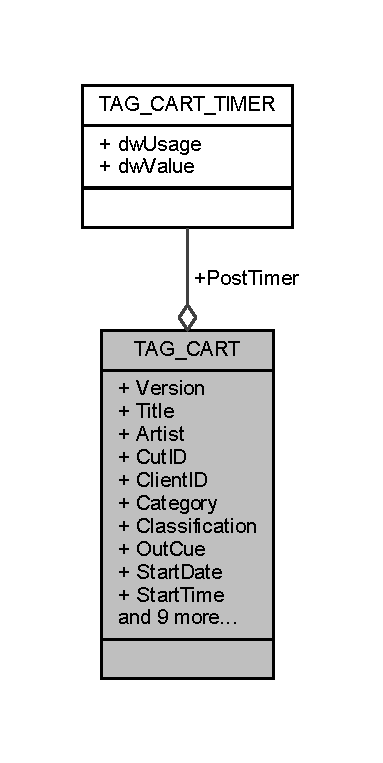
\includegraphics[width=184pt]{struct_t_a_g___c_a_r_t__coll__graph}
\end{center}
\end{figure}
\subsection*{Public Attributes}
\begin{DoxyCompactItemize}
\item 
\hypertarget{struct_t_a_g___c_a_r_t_ae0449a52a3967379de681b68423320bf_ae0449a52a3967379de681b68423320bf}{char {\bfseries Version} \mbox{[}4\mbox{]}}\label{struct_t_a_g___c_a_r_t_ae0449a52a3967379de681b68423320bf_ae0449a52a3967379de681b68423320bf}

\item 
\hypertarget{struct_t_a_g___c_a_r_t_a9045e907efbcce0931c91b3d6379d51a_a9045e907efbcce0931c91b3d6379d51a}{char {\bfseries Title} \mbox{[}64\mbox{]}}\label{struct_t_a_g___c_a_r_t_a9045e907efbcce0931c91b3d6379d51a_a9045e907efbcce0931c91b3d6379d51a}

\item 
\hypertarget{struct_t_a_g___c_a_r_t_a89be6e26acc15fd5a89cb472904a54f2_a89be6e26acc15fd5a89cb472904a54f2}{char {\bfseries Artist} \mbox{[}64\mbox{]}}\label{struct_t_a_g___c_a_r_t_a89be6e26acc15fd5a89cb472904a54f2_a89be6e26acc15fd5a89cb472904a54f2}

\item 
\hypertarget{struct_t_a_g___c_a_r_t_a18f64eef02546c78040a1695f3540868_a18f64eef02546c78040a1695f3540868}{char {\bfseries Cut\-I\-D} \mbox{[}64\mbox{]}}\label{struct_t_a_g___c_a_r_t_a18f64eef02546c78040a1695f3540868_a18f64eef02546c78040a1695f3540868}

\item 
\hypertarget{struct_t_a_g___c_a_r_t_a934296fdd35a3a235a0077803807d927_a934296fdd35a3a235a0077803807d927}{char {\bfseries Client\-I\-D} \mbox{[}64\mbox{]}}\label{struct_t_a_g___c_a_r_t_a934296fdd35a3a235a0077803807d927_a934296fdd35a3a235a0077803807d927}

\item 
\hypertarget{struct_t_a_g___c_a_r_t_ac1811370323a3b148124db4ce16aa6d9_ac1811370323a3b148124db4ce16aa6d9}{char {\bfseries Category} \mbox{[}64\mbox{]}}\label{struct_t_a_g___c_a_r_t_ac1811370323a3b148124db4ce16aa6d9_ac1811370323a3b148124db4ce16aa6d9}

\item 
\hypertarget{struct_t_a_g___c_a_r_t_abd83b077eed5262ce350518524650707_abd83b077eed5262ce350518524650707}{char {\bfseries Classification} \mbox{[}64\mbox{]}}\label{struct_t_a_g___c_a_r_t_abd83b077eed5262ce350518524650707_abd83b077eed5262ce350518524650707}

\item 
\hypertarget{struct_t_a_g___c_a_r_t_a032546411486b50dbb80fc9690227b64_a032546411486b50dbb80fc9690227b64}{char {\bfseries Out\-Cue} \mbox{[}64\mbox{]}}\label{struct_t_a_g___c_a_r_t_a032546411486b50dbb80fc9690227b64_a032546411486b50dbb80fc9690227b64}

\item 
\hypertarget{struct_t_a_g___c_a_r_t_a810bc5b4587b34a90eb4ea64fa9dfdfc_a810bc5b4587b34a90eb4ea64fa9dfdfc}{char {\bfseries Start\-Date} \mbox{[}10\mbox{]}}\label{struct_t_a_g___c_a_r_t_a810bc5b4587b34a90eb4ea64fa9dfdfc_a810bc5b4587b34a90eb4ea64fa9dfdfc}

\item 
\hypertarget{struct_t_a_g___c_a_r_t_a15980ecead3e2ff7754e830145825169_a15980ecead3e2ff7754e830145825169}{char {\bfseries Start\-Time} \mbox{[}8\mbox{]}}\label{struct_t_a_g___c_a_r_t_a15980ecead3e2ff7754e830145825169_a15980ecead3e2ff7754e830145825169}

\item 
\hypertarget{struct_t_a_g___c_a_r_t_ae7164e05a003bece0ef8dbe5092e394a_ae7164e05a003bece0ef8dbe5092e394a}{char {\bfseries End\-Date} \mbox{[}10\mbox{]}}\label{struct_t_a_g___c_a_r_t_ae7164e05a003bece0ef8dbe5092e394a_ae7164e05a003bece0ef8dbe5092e394a}

\item 
\hypertarget{struct_t_a_g___c_a_r_t_a07dca1b74291810968b11dc47c3e67b5_a07dca1b74291810968b11dc47c3e67b5}{char {\bfseries End\-Time} \mbox{[}8\mbox{]}}\label{struct_t_a_g___c_a_r_t_a07dca1b74291810968b11dc47c3e67b5_a07dca1b74291810968b11dc47c3e67b5}

\item 
\hypertarget{struct_t_a_g___c_a_r_t_ac97e4c02e22f3228b83d0a422c5c08b7_ac97e4c02e22f3228b83d0a422c5c08b7}{char {\bfseries Producer\-App\-I\-D} \mbox{[}64\mbox{]}}\label{struct_t_a_g___c_a_r_t_ac97e4c02e22f3228b83d0a422c5c08b7_ac97e4c02e22f3228b83d0a422c5c08b7}

\item 
\hypertarget{struct_t_a_g___c_a_r_t_a3b8c1e40668429cb8bbfeaf73c4c7068_a3b8c1e40668429cb8bbfeaf73c4c7068}{char {\bfseries Producer\-App\-Version} \mbox{[}64\mbox{]}}\label{struct_t_a_g___c_a_r_t_a3b8c1e40668429cb8bbfeaf73c4c7068_a3b8c1e40668429cb8bbfeaf73c4c7068}

\item 
\hypertarget{struct_t_a_g___c_a_r_t_ad2f48ed3ea41004894da01f6d4ac4135_ad2f48ed3ea41004894da01f6d4ac4135}{char {\bfseries User\-Def} \mbox{[}64\mbox{]}}\label{struct_t_a_g___c_a_r_t_ad2f48ed3ea41004894da01f6d4ac4135_ad2f48ed3ea41004894da01f6d4ac4135}

\item 
\hypertarget{struct_t_a_g___c_a_r_t_a3776ebc4bdd93cbfc5bb08e101a508fa_a3776ebc4bdd93cbfc5bb08e101a508fa}{D\-W\-O\-R\-D {\bfseries dw\-Level\-Reference}}\label{struct_t_a_g___c_a_r_t_a3776ebc4bdd93cbfc5bb08e101a508fa_a3776ebc4bdd93cbfc5bb08e101a508fa}

\item 
\hypertarget{struct_t_a_g___c_a_r_t_af0e070947244da684158dc1de513a2d1_af0e070947244da684158dc1de513a2d1}{\hyperlink{struct_t_a_g___c_a_r_t___t_i_m_e_r}{T\-A\-G\-\_\-\-C\-A\-R\-T\-\_\-\-T\-I\-M\-E\-R} {\bfseries Post\-Timer} \mbox{[}8\mbox{]}}\label{struct_t_a_g___c_a_r_t_af0e070947244da684158dc1de513a2d1_af0e070947244da684158dc1de513a2d1}

\item 
\hypertarget{struct_t_a_g___c_a_r_t_a38493fd6de87cc11b4764f72e97f2345_a38493fd6de87cc11b4764f72e97f2345}{char {\bfseries Reserved} \mbox{[}276\mbox{]}}\label{struct_t_a_g___c_a_r_t_a38493fd6de87cc11b4764f72e97f2345_a38493fd6de87cc11b4764f72e97f2345}

\item 
\hypertarget{struct_t_a_g___c_a_r_t_ae320e3568130ab502f0a552200029495_ae320e3568130ab502f0a552200029495}{char {\bfseries U\-R\-L} \mbox{[}1024\mbox{]}}\label{struct_t_a_g___c_a_r_t_ae320e3568130ab502f0a552200029495_ae320e3568130ab502f0a552200029495}

\item 
\hypertarget{struct_t_a_g___c_a_r_t_a5001ddf47b6e12aca5781d6420bbfe75_a5001ddf47b6e12aca5781d6420bbfe75}{char {\bfseries Tag\-Text} \mbox{[}$\,$\mbox{]}}\label{struct_t_a_g___c_a_r_t_a5001ddf47b6e12aca5781d6420bbfe75_a5001ddf47b6e12aca5781d6420bbfe75}

\end{DoxyCompactItemize}


\subsection{Detailed Description}


Definition at line 659 of file bass.\-h.



The documentation for this struct was generated from the following files\-:\begin{DoxyCompactItemize}
\item 
D\-A\-W\-Components/bass.\-h\item 
M\-S\-Master\-Cmp/bass.\-h\end{DoxyCompactItemize}

\hypertarget{struct_t_a_g___c_a_r_t___t_i_m_e_r}{\section{T\-A\-G\-\_\-\-C\-A\-R\-T\-\_\-\-T\-I\-M\-E\-R Struct Reference}
\label{struct_t_a_g___c_a_r_t___t_i_m_e_r}\index{T\-A\-G\-\_\-\-C\-A\-R\-T\-\_\-\-T\-I\-M\-E\-R@{T\-A\-G\-\_\-\-C\-A\-R\-T\-\_\-\-T\-I\-M\-E\-R}}
}


Collaboration diagram for T\-A\-G\-\_\-\-C\-A\-R\-T\-\_\-\-T\-I\-M\-E\-R\-:\nopagebreak
\begin{figure}[H]
\begin{center}
\leavevmode
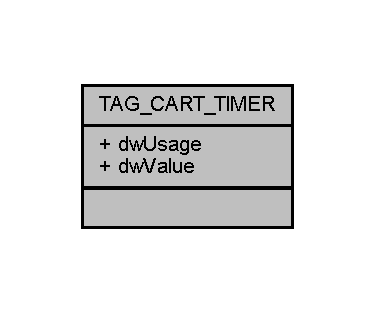
\includegraphics[width=180pt]{struct_t_a_g___c_a_r_t___t_i_m_e_r__coll__graph}
\end{center}
\end{figure}
\subsection*{Public Attributes}
\begin{DoxyCompactItemize}
\item 
\hypertarget{struct_t_a_g___c_a_r_t___t_i_m_e_r_aa40808e77b3759fe9126c02f027271d9_aa40808e77b3759fe9126c02f027271d9}{D\-W\-O\-R\-D {\bfseries dw\-Usage}}\label{struct_t_a_g___c_a_r_t___t_i_m_e_r_aa40808e77b3759fe9126c02f027271d9_aa40808e77b3759fe9126c02f027271d9}

\item 
\hypertarget{struct_t_a_g___c_a_r_t___t_i_m_e_r_aa5bbaed34d05a4febf635a1a46fe72b0_aa5bbaed34d05a4febf635a1a46fe72b0}{D\-W\-O\-R\-D {\bfseries dw\-Value}}\label{struct_t_a_g___c_a_r_t___t_i_m_e_r_aa5bbaed34d05a4febf635a1a46fe72b0_aa5bbaed34d05a4febf635a1a46fe72b0}

\end{DoxyCompactItemize}


\subsection{Detailed Description}


Definition at line 653 of file bass.\-h.



The documentation for this struct was generated from the following files\-:\begin{DoxyCompactItemize}
\item 
D\-A\-W\-Components/bass.\-h\item 
M\-S\-Master\-Cmp/bass.\-h\end{DoxyCompactItemize}

\hypertarget{struct_t_a_g___i_d3}{\section{T\-A\-G\-\_\-\-I\-D3 Struct Reference}
\label{struct_t_a_g___i_d3}\index{T\-A\-G\-\_\-\-I\-D3@{T\-A\-G\-\_\-\-I\-D3}}
}


Collaboration diagram for T\-A\-G\-\_\-\-I\-D3\-:\nopagebreak
\begin{figure}[H]
\begin{center}
\leavevmode
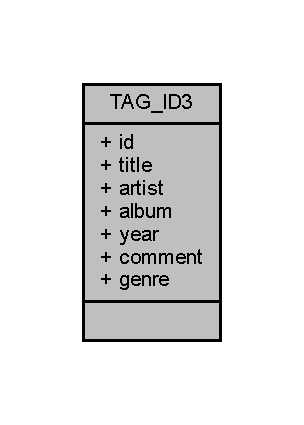
\includegraphics[width=146pt]{struct_t_a_g___i_d3__coll__graph}
\end{center}
\end{figure}
\subsection*{Public Attributes}
\begin{DoxyCompactItemize}
\item 
\hypertarget{struct_t_a_g___i_d3_acffd35f6f754060dc8b467b6d11c8068_acffd35f6f754060dc8b467b6d11c8068}{char {\bfseries id} \mbox{[}3\mbox{]}}\label{struct_t_a_g___i_d3_acffd35f6f754060dc8b467b6d11c8068_acffd35f6f754060dc8b467b6d11c8068}

\item 
\hypertarget{struct_t_a_g___i_d3_a18676a1bba83004481aa6a11d3d49dc5_a18676a1bba83004481aa6a11d3d49dc5}{char {\bfseries title} \mbox{[}30\mbox{]}}\label{struct_t_a_g___i_d3_a18676a1bba83004481aa6a11d3d49dc5_a18676a1bba83004481aa6a11d3d49dc5}

\item 
\hypertarget{struct_t_a_g___i_d3_a2bb38e8cc712fea72edc5678e8b7fc64_a2bb38e8cc712fea72edc5678e8b7fc64}{char {\bfseries artist} \mbox{[}30\mbox{]}}\label{struct_t_a_g___i_d3_a2bb38e8cc712fea72edc5678e8b7fc64_a2bb38e8cc712fea72edc5678e8b7fc64}

\item 
\hypertarget{struct_t_a_g___i_d3_a24dd09e6778d26698854747ac1cce0b9_a24dd09e6778d26698854747ac1cce0b9}{char {\bfseries album} \mbox{[}30\mbox{]}}\label{struct_t_a_g___i_d3_a24dd09e6778d26698854747ac1cce0b9_a24dd09e6778d26698854747ac1cce0b9}

\item 
\hypertarget{struct_t_a_g___i_d3_a1792effd9f4ea0bb1bd2cbca42859512_a1792effd9f4ea0bb1bd2cbca42859512}{char {\bfseries year} \mbox{[}4\mbox{]}}\label{struct_t_a_g___i_d3_a1792effd9f4ea0bb1bd2cbca42859512_a1792effd9f4ea0bb1bd2cbca42859512}

\item 
\hypertarget{struct_t_a_g___i_d3_acbd96db32112f3afb5c5b350e8005d9d_acbd96db32112f3afb5c5b350e8005d9d}{char {\bfseries comment} \mbox{[}30\mbox{]}}\label{struct_t_a_g___i_d3_acbd96db32112f3afb5c5b350e8005d9d_acbd96db32112f3afb5c5b350e8005d9d}

\item 
\hypertarget{struct_t_a_g___i_d3_af7a5412ae2d2acafd300dca3212dbbc2_af7a5412ae2d2acafd300dca3212dbbc2}{B\-Y\-T\-E {\bfseries genre}}\label{struct_t_a_g___i_d3_af7a5412ae2d2acafd300dca3212dbbc2_af7a5412ae2d2acafd300dca3212dbbc2}

\end{DoxyCompactItemize}


\subsection{Detailed Description}


Definition at line 609 of file bass.\-h.



The documentation for this struct was generated from the following files\-:\begin{DoxyCompactItemize}
\item 
D\-A\-W\-Components/bass.\-h\item 
M\-S\-Master\-Cmp/bass.\-h\end{DoxyCompactItemize}

\hypertarget{structt_w_a_v_e_f_o_r_m_a_t_e_x}{\section{t\-W\-A\-V\-E\-F\-O\-R\-M\-A\-T\-E\-X Struct Reference}
\label{structt_w_a_v_e_f_o_r_m_a_t_e_x}\index{t\-W\-A\-V\-E\-F\-O\-R\-M\-A\-T\-E\-X@{t\-W\-A\-V\-E\-F\-O\-R\-M\-A\-T\-E\-X}}
}


Collaboration diagram for t\-W\-A\-V\-E\-F\-O\-R\-M\-A\-T\-E\-X\-:\nopagebreak
\begin{figure}[H]
\begin{center}
\leavevmode
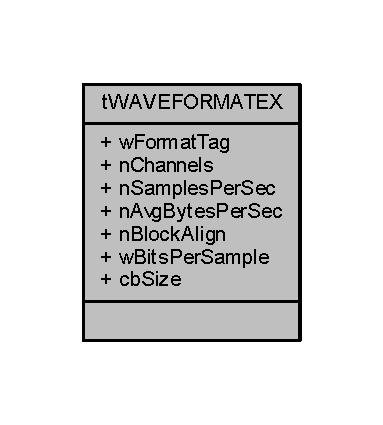
\includegraphics[width=184pt]{structt_w_a_v_e_f_o_r_m_a_t_e_x__coll__graph}
\end{center}
\end{figure}
\subsection*{Public Attributes}
\begin{DoxyCompactItemize}
\item 
\hypertarget{structt_w_a_v_e_f_o_r_m_a_t_e_x_aec624a88d0d94d7789c60dcc1418d6fc_aec624a88d0d94d7789c60dcc1418d6fc}{W\-O\-R\-D {\bfseries w\-Format\-Tag}}\label{structt_w_a_v_e_f_o_r_m_a_t_e_x_aec624a88d0d94d7789c60dcc1418d6fc_aec624a88d0d94d7789c60dcc1418d6fc}

\item 
\hypertarget{structt_w_a_v_e_f_o_r_m_a_t_e_x_ae71090e815279542a4f2ffea72ff1a07_ae71090e815279542a4f2ffea72ff1a07}{W\-O\-R\-D {\bfseries n\-Channels}}\label{structt_w_a_v_e_f_o_r_m_a_t_e_x_ae71090e815279542a4f2ffea72ff1a07_ae71090e815279542a4f2ffea72ff1a07}

\item 
\hypertarget{structt_w_a_v_e_f_o_r_m_a_t_e_x_ad3a2f0a0aed0d8b3a5f6afad5f8b6acc_ad3a2f0a0aed0d8b3a5f6afad5f8b6acc}{D\-W\-O\-R\-D {\bfseries n\-Samples\-Per\-Sec}}\label{structt_w_a_v_e_f_o_r_m_a_t_e_x_ad3a2f0a0aed0d8b3a5f6afad5f8b6acc_ad3a2f0a0aed0d8b3a5f6afad5f8b6acc}

\item 
\hypertarget{structt_w_a_v_e_f_o_r_m_a_t_e_x_a933a772d450a8a8939fc96d1eb15c672_a933a772d450a8a8939fc96d1eb15c672}{D\-W\-O\-R\-D {\bfseries n\-Avg\-Bytes\-Per\-Sec}}\label{structt_w_a_v_e_f_o_r_m_a_t_e_x_a933a772d450a8a8939fc96d1eb15c672_a933a772d450a8a8939fc96d1eb15c672}

\item 
\hypertarget{structt_w_a_v_e_f_o_r_m_a_t_e_x_abb977590324e3d1b5a14f94b806b8ec1_abb977590324e3d1b5a14f94b806b8ec1}{W\-O\-R\-D {\bfseries n\-Block\-Align}}\label{structt_w_a_v_e_f_o_r_m_a_t_e_x_abb977590324e3d1b5a14f94b806b8ec1_abb977590324e3d1b5a14f94b806b8ec1}

\item 
\hypertarget{structt_w_a_v_e_f_o_r_m_a_t_e_x_a888d33f1b1415c903bfa95ebedc78516_a888d33f1b1415c903bfa95ebedc78516}{W\-O\-R\-D {\bfseries w\-Bits\-Per\-Sample}}\label{structt_w_a_v_e_f_o_r_m_a_t_e_x_a888d33f1b1415c903bfa95ebedc78516_a888d33f1b1415c903bfa95ebedc78516}

\item 
\hypertarget{structt_w_a_v_e_f_o_r_m_a_t_e_x_a179487978b7d541067d6200524ceff2c_a179487978b7d541067d6200524ceff2c}{W\-O\-R\-D {\bfseries cb\-Size}}\label{structt_w_a_v_e_f_o_r_m_a_t_e_x_a179487978b7d541067d6200524ceff2c_a179487978b7d541067d6200524ceff2c}

\end{DoxyCompactItemize}


\subsection{Detailed Description}


Definition at line 702 of file bass.\-h.



The documentation for this struct was generated from the following files\-:\begin{DoxyCompactItemize}
\item 
D\-A\-W\-Components/bass.\-h\item 
M\-S\-Master\-Cmp/bass.\-h\end{DoxyCompactItemize}

\addcontentsline{toc}{part}{Index}
\printindex
\end{document}
